\chapter{Using Uintah} \label{Chapter:UCF}

Several executable programs have been developed using the Uintah
Computational Framework (UCF).  The primary code that drives the
components implemented in Uintah is called \tt sus, \normalfont which
stands for Standalone Uintah Simulation.  The existing components were
originally developed to solve a complex fluid structure problem
involving a container filled with an explosive enveloped in a fire.

The code models the fire and the subsequent heat transfer to the
container followed by the resultant container deformation and ultimate
rupture due to the ignition and burning of the explosive material all
running on thousands of processors requiring thousands of hours of
computer time and hundreds of gigabytes of data storage.  Although
Uintah was developed originally to solve this complicated
multi-physics problem, the general nature of the algorithms and the
framework have allowed researchers to use the code to investigate a
wide range of problems.  The framework is general purpose enough to
allow for the implementation of a variety of implicit and explicit
algorithms on structured grids.  In addition, particle based
algorithms can be implemented using the native particle support found
in the framework.

This code leverages the task based parallelism inherent in the UCF to
implement several time stepping algorithms for structural mechanics,
fluid dynamics, and fluid structure interactions.  What follows is a
description of using \tt sus \normalfont within the realm of
structural mechanics, fluid mechanics, and structure-fluid
interactions.

\section{Installing the Uintah Software}

For information on downloading the Uintah software package (via
tarball or SVN), and how to setup (configure) and build (make) the
system, please refer to the Uintah Installation Guide.

%__________________________________
\section{Mechanics of Running sus}

For single processor simulations, the \tt sus \normalfont executable
(Standalone Uintah Simulation) is run from the command line prompt
like this:
\begin{Verbatim}[fontsize=\footnotesize]
  sus input.ups
\end{Verbatim}
where \tt input.ups \normalfont is an XML formatted input file.  The
Uintah software release contains numerous example input files located
in the \tt src/StandAlone/inputs/UintahRelease \normalfont directory.

For multiprocessor runs, the user generally uses \tt mpirun
\normalfont to launch the code.  Depending on the environment, batch
scheduler, launch scripts, etc, \tt mpirun \normalfont may or may not
be used.  However, in general, something like the following is used:
\begin{Verbatim}[fontsize=\footnotesize]
  mpirun -np num_processors sus -mpi input.ups
\end{Verbatim}

\tt num\_processors \normalfont is the number of processors that will
be used.  The input file must contain a patch layout that has at least
the same number (or greater) of patches as processors specified by a
number following the -np option shown above.

In addition, the \tt -mpi \normalfont is optional but often times
necessary if the mpi environment is not automatically detected from
within the sus executable.

Uintah provides for restarting from checkpoint as well.  For information on
this, see Section~\ref{Sec:DataArchiver}, which describes how to create
checkpoint data, and how to restart from it.

\section{Uintah Problem Specification (UPS)} \label{Sec:UPS}

The Uintah framework uses XML like input files to specify the various
parameters required by simulation components.  These Uintah Problem
Specification (.ups) files are validated based on the specification
found in \tt src/StandAlone/inputs/UPS\_SPEC/ups\_spec.xml \normalfont
(and its sibling files).  

The application developer is free to use any of the specified tags to
specify the data needed by the simulation.  The essential tags that
are required by Uintah include the following:

\begin{Verbatim}[fontsize=\footnotesize]
  <Uintah_specification>

  <SimulationComponent>

  <Time>

  <DataArchiver>

  <Grid>
\end{Verbatim}


Individual components have additional tags that specify properties,
algorithms, materials, etc. that are unique to that individual
components.  Within the individual sections on MPM, ICE, MPMICE,
Arches, and MPMArches, the individual tags will be explained more
fully.

The sus executable verifies that the input file adheres to a consistent
specification and that all necessary tags are specified.  However, it
is up to the individual creating or modifying the input file to put in
physically reasonable set of consistent parameters.


\section{Simulation Components} \label{Sec:SimulationComponent}

The input file tag for SimulationComponent has the \tt type \normalfont
attribute that must be specified with either \tt mpm, mpmice, ice, arches,
\normalfont or \tt mpmarches, \normalfont as in:

\begin{Verbatim}[fontsize=\footnotesize]
<SimulationComponent type = "mpm" />
\end{Verbatim}



%__________________________________
\section{Time Related Variables} \label{Sec:TimeRelatedVariables}
Uintah components are time dependent codes.  As such, one of the first
entries in each input file describes the time-stepping parameters.  An
input file segment is given below that encompasses all of the possible
parameters.  The function of each of these parameters is described below.

\begin{Verbatim}[fontsize=\footnotesize]
<Time>
    <maxTime>            1.0         </maxTime>
    <initTime>           0.0         </initTime>
    <delt\_min>           0.0         </delt\_min>
    <delt\_max>           1.0         </delt\_max>
    <delt\_init>          1.0e-9      </delt\_init>
    <max\_delt\_increase>  2.0         </max\_delt\_increase>
    <timestep\_multiplier>1.0         </timestep\_multiplier>
    <max\_Timestep>       100         </max\_Timestep>
    <end\_on\_max\_time\_exactly>true    </end\_on\_max\_time\_exactly>
</Time>
\end{Verbatim}

The following fields are required:

\begin{itemize}
\item maxTime - how long in physical time to run the simulation for
\item initTime - what time to begin the simulation at
\item delt\_min - the smallest timestep the simulation will take
\item delt\_max - the largest timestep the simulation will take
\item timestep\_multiplier - multiplies the timestep by this number (before adjusting to min or max timestep)
\end{itemize}

The following fields are optional:

\begin{itemize}
\item delt\_init - The timestep to take initially (assuming it's less than the one computed by the simulation)
\item initial\_delt\_range - The period of time to use the delt\_init (default = 0)
\item max\_delt\_increase - Maximum amount to multiply the previous delt by (if the newly computed delt is greater than the previous one)
\item max\_iterations - The number of timesteps to run the simulation for (even on a restart)
\item max\_Timesteps - The timestep number to end the simulation on (not usually used with max\_iterations)
\item override\_restart\_delt - On a restart, use this delt instead of the most-recently-used delt.
\item clamp\_timesteps\_to\_output - Sync the delt with the DataArchiver - when an output timestep occurs, reduce the delt to have the time land on the timestep interval (default = false)
\item end\_on\_max\_time\_exactly - clamp the delt such that the last timesteps end on what was specified in maxTime (default = false)
\end{itemize}

A word about timesteps: In general, the timestep (delt) is computed at various stages within a timestep, and the smallest one is used, unless it needs to raise the delt to the delt\_min.




%
%__________________________________
\section{Data Archiver} \label{Sec:DataArchiver}

The Data Archiver section specifies the directory name where data will
be stored and what variables will be saved and how often data is saved
and how frequently the simulation is checkpointed.

The \tt <filebase> \normalfont tag is used to specify the directory
name and by convention, the \tt .uda \normalfont suffix is attached denoting the
``Uintah Data Archive".

Data can be saved based on a frequency setting that is either based on time
intervals;\\
\tt <outputTimestepInterval> integer\_number\_of\_steps </outputTimestepInterval> \normalfont\\
or timestep intervals; \\
\tt <outputInterval> floating\_point\_time\_increment </outputInterval> \normalfont\\

Each simulation component specifies variables with label names that
can be specified for data output.  By convention, particle data are
denoted by \tt p. \normalfont followed by a particular variable name
such as mass, velocity, stress, etc.  Whereas for node based data, the
convention is to use the \tt g. \normalfont followed by the variable
name, such as mass, stress, velocity, etc.  Similarly, cell-centered
and face-centered data typically end with the a trailing \tt CC \normalfont
or \tt FC, \normalfont  respectively.  Within the DataArchiver
section, variables are specified with the following format:

\begin{Verbatim}[fontsize=\footnotesize]
   <save label = "p.mass" />
   <save label = "g.mass" />
\end{Verbatim}

To see a list of
variables available for saving for a given component, execute the following
command from the \tt StandAlone \normalfont directory:

\begin{Verbatim}[fontsize=\footnotesize]
inputs/labelNames component
\end{Verbatim}
where \TT{component} is, e.g., \TT{mpm}, \TT{ice,} etc.

Check-pointing information can be created that provides a mechanism for
restarting a simulation at a later point in time.  The \TT{<checkpoint>}
tag with the \TT{cycle} and \TT{ interval} attributes describe how many
copies of checkpoint data is stored (cycle) and how often it is generated
(interval).  You may also use the \TT{walltimeStart} and \TT{walltimeInterval}
options for specifying when and how offen a checkpoint will be output based
on wall-clock time.

As an example of checkpoint data that has two timesteps worth of
che dckpoint data that is created every .01 seconds of simulation time
are shown below:

\begin{Verbatim}[fontsize=\footnotesize]
<checkpoint cycle = "2" interval = "0.01"/>
\end{Verbatim}
% d

To restart from a checkpointed archive, simply put ``\tt -restart\normalfont" in the
sus command-line arguments and specify the .uda directory instead of
a ups file (sus reads the copied \tt input.xml \normalfont from the
archive).  One can optionally specify a certain timestep to restart
from with \tt -t timestep \normalfont with multiple checkpoints, but the
last checkpointed timestep is the default.  When restarting, sus
copies all of the appropriate information from the old uda directory to its
new uda directory.
% I'M NOT SURE ABOUT THIS, -nocopy REMOVES THE OLD UDA?  I THOUGHT IT
% JUST LEFT STUFF IN THE OLD UDA, WHERE AS -copy MADE A COPY OF OLD TIMESTEP
% DATA, AND -move MOVED THE OLD TIMESTEP DATA TO THE NEW UDA.  
%  If one doesn't want to keep the old uda directory
%around, they can specify \tt -nocopy \normalfont to have it be removed
%(e.g., if you are cramped for disk space).  Either way it creates a new uda
%directory for you as always.

Here are some examples:

\begin{Verbatim}[fontsize=\footnotesize]
./sus -mpm -restart disks.uda.000 -nocopy
./sus -mpm -restart disks.uda.000 -t 29
\end{Verbatim}
%
%__________________________________

\section{Simulation Options} \label{Sec:SimulationOptions}


There are many options available when running MPM simulations.  These
are generally specified in the \tt <MPM> \normalfont section of the input file.
A list of these options taken from 
\tt inputs/UPS\_SPEC/mpm\_spec.xml \normalfont  is given in section \ref{Sec:UintahImp}.

\section{Geometry objects} \label{Sec:GeometryObjects}

Within several of the components, the material is described by a
combination of physical parameters and the geometry.  Geometry objects
use the notion of constructive solid geometry operations to compose
the layout of the material from simple shapes such as boxes, spheres,
cylinders and cones, as well as operators which include the union,
intersections, differences of the simple shapes.  In addition to the
simple shapes, triangulated surfaces can be used in conjunction with
the simple shapes and the operations on these shapes.

Each geometry object has the following properties, label (string
name), type (box, cylinder, sphere, etc), resolution (vector
quantity), and any unique geometry parameters such as origin, corners,
triangulated data file, etc.  The operators which include, the union,
the difference, and intersection tags contain either lists of
additional operators or the primitives pieces.

As an example of a non-trivial geometry object is shown below:

\begin{Verbatim}[fontsize=\footnotesize]
<geom_object>
     <intersection>
       <box label = "Domain">
          <min>[0.0,0.0,0.0]</min>
          <max>[0.1,0.1,0.1]</max>
       </box>
       <union>
         <sphere label = "First node">
            <origin>[0.022,0.028,0.1  ]</origin>
            <radius>0.01</radius>
         </sphere>
         <sphere label = "2nd node">
            <origin>[0.030,0.075,0.1  ]</origin>
            <radius>0.01</radius>
         </sphere>
       </union>
     </intersection>
     <res>[2,2,2]</res>
     <velocity>[0.,0.,0.]</velocity>
     <temperature>0 </temperature>
</geom_object>
\end{Verbatim}

The following geometry objects are given with their required tags:

\tt box \normalfont has the following tags: min and max which are
vector quantities specified in the \tt [a, b, c] \normalfont format.

\tt sphere \normalfont has an origin tag specified as a vector and the
radius tag specified as a float.

\tt cone \normalfont has a tag for the top and bottom origins (vector)
as well as tags for the top and bottom radius (float) to create a
right circular cone/frustum.

\tt cylinder \normalfont has a tag for the top and bottom origins
(vector) plus a tag for the radius (float).

\tt smoothcyl \normalfont is a geomtry object designed for use with
the cpdi algorithm, which uses a body fit particle spatial
distribution.  This eliminates ``stair-stepped'' boundaries typical of
the standard, grid-based, discretization scheme.  Thus {\it it is
  important to note that this geometry is only designed to work with
  \tt <interpolator>cpdi</interpolator>\normalfont. \it Other
  algorithms may give erroneous answers.}

This geometry has the following tags:

\begin{Verbatim}[fontsize=\footnotesize]
	   <smoothcyl label = "label name">
	     <discretization_scheme> string </discretization_scheme>
	     <bottom> vector </bottom>
	     <top> vector </top>
	     <outer_radius> float </outer_radius>
	     <inner_radius> float </inner_radius>
	     <num_radial> integer </num_radial>
	     <num_axial> integer </num_axial>
	     <num_angular> integer </num_angular>
	     <arc_start_angle> double (in degrees) </arc_start_angle>
	     <arc_angle> double (in degrees) </arc_angle>
	   </smoothcyl>
\end{Verbatim}

The complete or partial annulus or cylinder specified by inner
(optional, defaulting to zero) and outer radii, cylinder axis bottom
and top (all required) and start and final angle (both optional,
defaulting to 0 and 360) will be discretized using planes of
concentric rings of particles.  Particle density is specified by \tt
num\_axial \normalfont and \tt num\_radial\normalfont, the number of
particles in the axial and radial dimensions, respectively
\normalfont.  Note that these particle density specifications
supercede those specified in the \tt <geom\_object> <res> \normalfont
tag, which is ignored.

The required discretization scheme may be either \tt pie\_slices
\normalfont or \tt constant\_particle\_volumes\normalfont.  For the
\tt pie\_slices \normalfont discretization, \tt num\_angular
\normalfont is required to specify the number of particles between \tt
arc\_start \normalfont and \tt arc\_angle \normalfont.  For the \tt
constant\_particle\_volumes \normalfont discretization, the number of
particles between \tt arc\_start \normalfont and \tt arc\_angle
\normalfont is determined individually for each ring of particles by
attempting to keep particle spacings approximately equal in the radial
and angular directions, and thus particle volumes approximately
constant.

End caps may be added to the smoothcyl using the optional \tt
<endcap\_thickness> \normalfont tag, which specifies the axial
dimension of cylinders which are appended to each end of the specified
\tt smoothcyl\normalfont (the radii are the same as the \tt smoothcyl
\normalfont).  Presently, the end cap body fit discretization uses a
legacy scheme.

Note: At the time of writing, multiple \tt smoothcyl \normalfont
geometries within a \tt <geom\_object> \normalfont tag were not
discretized using a body fit particle distribution as described here
(rather the default discretization scheme is used).  This will be
fixed eventually, at which point it may be possible to create more
general endcaps using unions of \tt smoothcyl \normalfont.

\tt ellipsoid \normalfont has an origin tag specified as a vector.  There are 
two ways to assign axis lengths depending on the orientation of the ellipsoid.
If the axes are aligned with the Cartesian grid, they may be specified as 
floating point values with tagnames: rx, ry, rz.  For all other orientation, 
three vector quantities must be specified in the \tt [a,b,c] \normalfont format.
Vector quantity tag names are: v1, v2, v3.These vectors must be orthogonal 
to within 1e-12 after dot product or the simulation will throw an exception.  
Note, if both vector quantities and floating point tags are used, 
the vector quantity inputs will take precedence.  

\tt parallelepiped \normalfont requires that four points be specified as
illustrated by the ASCII art snippet taken from the source code:

\begin{Verbatim}[fontsize=\footnotesize]
//********************************************
//                                          //
//             *-------------*              //
//            / .           / \             //
//           /   .         /   \            //
//          P4-------------*    \           //
//           \    .         \    \          //
//            \   P2.........\....*         //
//             \ .            \  /          //
//             P1--------------P3           //
//
//  Returns true if the point is inside (or on) the parallelepiped.
//  (The order of p2, p3, and p4 doesn't really matter.)
\end{Verbatim}

\tt tri \normalfont is a tag for describing a triangulated surface.
The name tag specifies the file name to use for reading in the
triangulated surface description and the points file.  The
triangulated surface (file\_name.tri) contains a list of integers
describing the connectivity of points specified in file\_name.pts.
Here is an excerpt from a tri file and a points file:

\begin{Verbatim}[fontsize=\footnotesize]
Triangulated file

1 39 41
1 41 38
38 41 42
. . .

Points file

0 0.03863 -0.005
0.35227 0.13023 -0.005
0.00403479 0.0296797 -0.005
. . .
\end{Verbatim}
The Mach 2 Wedge example in Section~\ref{Sec:MPMICE_EXAMPLES} depicts usage of
this option.

The boolean operators on the geometry pieces include \tt difference,
intersection, \normalfont and \tt union.\normalfont

The \tt difference \normalfont takes two geometry pieces and subtracts
the second geometry piece from the first geometry piece.  The \tt
intersection \normalfont operator requires at least two geometry
pieces in forming an intersection geometry piece.  Whereas the \tt
union \normalfont operator aggregates a collection of geometry pieces.
Multiple operators can be used to form very complex geometry pieces.

An additional input in the \tt <geom\_object> \normalfont field is the
\tt <res> \normalfont tag.  In MPM, this simply refers to how many particles
are placed in each cell in each coordinate direction.  For multi-material ICE
simulations, the \tt <res> \normalfont serves a similar purpose in that one
can specify the subgrid resolution of the initial material distribution
of mixed cells at the interface of geometry objects.

In addition to the above, it is also possible in MPM simulations to describe
geometry by providing a file containing a series of particle locations.  These
can be in either ASCII or binary format.  In addition, it is also possible to
provide initial data for certain variables on the particles, including
volume, temperature, external force, fiber direction (used in material models
with transverse isotropy) and velocity.  The following is an example in which
external force and fiber direction are specified:

\begin{Verbatim}[fontsize=\footnotesize]
          <file>
              <name>LVcoarse.pts</name>
              <var>p.externalforce</var>
              <var>p.fiberdir</var>
          </file>
\end{Verbatim}

where the text file LVcoarse.pts looks like:

\begin{Verbatim}[fontsize=\footnotesize]
0.0385 0.0335 0.0015 0 0 0 0.248865 -0.0593421 -0.966718
0.0395 0.0335 0.0015 0 0 0 0.254892 -0.0220365 -0.966718
0.0405 0.0335 0.0015 0 0 0 0.267002 0.0197728 -0.963493
0.0415 0.0335 0.0015 0 0 0 0.261177 0.0588869 -0.963493
	.
	.
	.
\end{Verbatim}
Because these files can be arbitrarily large, an additional preprocessing step
must be taken before issuing the \tt sus \normalfont command.
\tt pfs \normalfont for ``Particle File Splitter" is a utility that splits the
data in the \tt .pts \normalfont file into a series of files
(\tt file.pts.0, file.pts.1, \normalfont, etc), one for each
patch.  By doing this, each processor needs only read in the data for the
patches that it contains, rather than each processor reading in the entire file,
which can be hard on the file system.  Note, that this step is required,
even if only using a single patch, and must be reissued any time the patch
configuration is changed.  Usage of this utility, which is compiled
into the \tt StandAlone/tools/pfs \normalfont directory, is:

\begin{Verbatim}[fontsize=\footnotesize]
   pfs input.ups
\end{Verbatim}

One final option is available for initializing particle positions in MPM
simulations, and that is through the use of three dimensional image data,
such as might be collected via CT scans or confocal microscopy.  The image data are provided as 8-bit raw files, and usage in the input file is given as:

\begin{Verbatim}[fontsize=\footnotesize]
        <image>
          <name>spheres.raw</name>
          <res>[1600, 1600, 1600]</res>
          <threshold>[1, 25]</threshold>
        </image>
        <file>
          <name>spheres.pts</name>
          <format>bin</format>
        </file>
\end{Verbatim}

The \tt <image> \normalfont section gives the name of the file, the resolution, in pixels,
in the various coordinate directions, and threshold range.  Particles will be
generated at voxels within the specified range.  The \tt <file> \normalfont
section is the same as that described above.  A different preprocessing utility
is provided when using image data (for the same reasons described previously).
Usage is as follows:

\begin{Verbatim}[fontsize=\footnotesize]
   pfs2 -b input.ups
\end{Verbatim}

The -b indicates that binary \tt spheres.pts.\# \normalfont files will be created, which
saves considerable disk space when performing large simulations.


%__________________________________
\section{Boundary conditions}\label{sec:ucf_bc}

Boundary conditions are specified within the \tt <Grid> \normalfont
but are described separately for clarity.  The essential idea is that
boundary conditions are specified on the domain of the grid.  Values
can be assigned either on the entire face, or parts of the face.
Combinations of various geometric descriptions are used to aid in the
assignment of values over specific regions of the grid.  Each of the
six faces of the grid is denoted by either the minus or plus side of
the domain.

The XML description of a particular boundary condition includes which
side of the domain, the material id, what type of boundary condition
(Dirichlet or Neumann) and which variable and the value assigned.  The
following is a an MPM specification of a Dirichlet boundary condition
assigned to the velocity component on the x minus face (the entire
side) with a vector value of [0.0,0.0,0.0] applied to all of the materials.

\begin{Verbatim}[fontsize=\footnotesize]

 <Grid>
       <BoundaryConditions>
         <Face side = "x-">
             <BCType id = "all" var = "Dirichlet" label = "Velocity">
                   <value> [0.0,0.0,0.0] </value>
             </BCType>
         </Face>
         <Face side = "x+">
            <BCType id = "all" var = "Dirichlet" label = "Velocity">
                 <value> [0.0,0.0,0.0] </value>
            </BCType>
         </Face>
        . . . .
        <BoundaryCondition>
   . . . .
  <Grid>

\end{Verbatim}

The notation \tt <Face side = "x-"> \normalfont indicates that the
entire x minus face of the boundary will have the boundary condition
applied.  The \tt id = "all" \normalfont means that all the
materials will have this value.  To specify the boundary condition for
a particular material, specify an integer number instead of the
"all".  The \tt var = "Dirichlet" \normalfont is used to specify
whether it is a Dirichlet or Neumann or symmetry boundary conditions.
Different components may use the \tt var \normalfont to include a
variety of different boundary conditions and are explained more fully
in the following component sections.  The \tt label = "Velocity"
\normalfont specifies which variable is being assigned and again is
component dependent.  The \tt <value> [0.0,0.0,0.0] </value>
\normalfont specifies the value.

An example of a more complicated boundary condition demonstrating a
hot jet of fluid issued into the domain is described.  The jet is
described by a circle on one side of the domain with boundary
conditions that are different in the circular jet compared to the rest
of the side.

\begin{Verbatim}[fontsize=\footnotesize]

 <Face circle = "y-" origin = "0.0 0.0 0.0" radius = ".5">
        <BCType id = "0"   label = "Pressure" var = "Neumann">
                              <value> 0.0   </value>
        </BCType>
        <BCType id = "0" label = "Velocity" var = "Dirichlet">
                              <value> [0.,1.,0.] </value>
        </BCType>
        <BCType id = "0" label = "Temperature" var = "Dirichlet">
                              <value> 1000.0  </value>
        </BCType>
        <BCType id = "0" label = "Density" var = "Dirichlet">
                              <value> .35379  </value>
        </BCType>
        <BCType id = "0" label = "SpecificVol"  var = "computeFromDensity">
                              <value> 0.0  </value>
        </BCType>
      </Face>
      <Face side = "y-">
        <BCType id = "0"   label = "Pressure"     var = "Neumann">
                              <value> 0.0   </value>
        </BCType>
        <BCType id = "0" label = "Velocity"     var = "Dirichlet">
                              <value> [0.,0.,0.] </value>
        </BCType>
        <BCType id = "0" label = "Temperature"  var = "Neumann">
                              <value> 0.0  </value>
        </BCType>
        <BCType id = "0" label = "Density"      var = "Neumann">
                              <value> 0.0  </value>
        </BCType>
        <BCType id = "0" label = "SpecificVol"  var = "computeFromDensity">
                              <value> 0.0  </value>
        </BCType>
      </Face>

\end{Verbatim}

The jet is described by the circle on the y minus face with the origin
at 0,0,0 and a radius of .5.  For the region outside of the circle,
the boundary conditions are different.  Each side must have at least
the \tt "side" \normalfont specified, but additional circles and
rectangles can be specified on a given face.

An example of the \tt rectangle \normalfont is specified as with the
lower corner at 0,0.181,0 and upper corner at 0,0.5,0.


\begin{Verbatim}[fontsize=\footnotesize]
 <Face rectangle = "x-" lower = "0.0 0.181 0.0" upper = "0.0 0.5 0.0">
\end{Verbatim}

%
%__________________________________
\section{Grid specification} \label{Sec:Grid}

The \tt <Grid> \normalfont section specifies the domain of the
structured grid and includes tags which indicate the lower and upper
corners, the number of extra cells which can be used by various
components for the application of boundary conditions or interpolation
schemes.  

The grid is decomposed into a number of patches.  For single processor
problems, usually one patch is used for the entire domain.  For
multiple processor simulations, there must be at least one patch per
processor.  Patches are specified along the x,y,z directions of the
grid using the \tt <patches> [2,5,3] </patches> \normalfont which
specifies two patches along the x direction, five patches along the y
direction and 3 patches along the z direction.  The maximum number of
processors that \tt sus \normalfont could use is $2*5*3 = 30$.
Attempting to use more processors than patches
will cause a run time error during initialization.

Finally, the grid spacing can specified using either a fixed number of
cells along each x,y,z direction or by the size of the grid cell in
each direction.  To specify a fixed number of grid cells, use the \tt
<resolution> [20,20,3] </resolution> \normalfont.  This specifies 20
grid cells in the x direction, 20 in the y direction and 3 in the z
direction.  To specify the grid cell size use the \tt <spacing>
[0.5,0.5,0.3] </spacing> \normalfont.  This specifies the a grid cell
size of .5 in the x and y directions and .3 in the z direction.  The
\tt <resolution> \normalfont and \tt <spacing> \normalfont cannot be
specified together.  The following two examples would generate
identical grids:

\begin{Verbatim}[fontsize=\footnotesize]
<Level>
    <Box label="1">
       <lower>        [0,0,0]          </lower>
       <upper>        [5,5,5]          </upper>
       <extraCells>   [1,1,1]          </extraCells>
       <patches>      [1,1,1]          </patches>
    </Box>
    <spacing>         [0.5,0.5,0.5]    </spacing>
</Level>
\end{Verbatim}

\begin{Verbatim}[fontsize=\footnotesize]
<Level>
    <Box label="1">
       <lower>        [0,0,0]          </lower>
       <upper>        [5,5,5]          </upper>
       <resolution>   [10,10,10]       </resolution>
       <extraCells>   [1,1,1]          </extraCells>
       <patches>      [1,1,1]          </patches>
    </Box>
</Level>
\end{Verbatim}


The above examples indicate that the grid domain has a lower corner at
0,0,0 and an upper corner at 5,5,5 with one extra cell in each
direction.  The domain is broken down into one patch covering the
entire domain with a grid spacing of .5,.5,.5.  Along each dimension
there are ten cells in the interior of the grid and one layer of
``extraCells" outside of the domain.  extraCells are the Uintah nomenclature
for what are frequently referred to as ``ghost-cells".

%
%__________________________________
%\section{Adaptive Mesh Refinement}
%- Describe refinement flags
%- Describe boundary layers
%- How is a cell flagged as needing to be refined
%
%__________________________________

\section{AMR} \label{Sec:AMR}

In general, the AMR input looks like:

\begin{Verbatim}[fontsize=\footnotesize]
  <AMR>
      <ICE>
        <do_Refluxing>        false    </do_Refluxing>
        <orderOfInterpolation>1         </orderOfInterpolation>
        <Refinement_Criteria_Thresholds>
          <Variable name = "press_CC" value = "1e6" matl = "0" />
        </Refinement_Criteria_Thresholds>
      </ICE>
      <MPM>
        <min_grid_level>-1</min_grid_level>
        <max_grid_level>-1</max_grid_level>
      </MPM>
      <useLockStep>true</useLockStep>
      <Regridder type="Tiled">
\end{Verbatim}

\begin{Verbatim}[fontsize=\footnotesize]
        <!--General Regridder Settings-->
        <max_levels>2</max_levels>
        <cell_refinement_ratio>    [[2,2,1]]</cell_refinement_ratio>
        <cell_stability_dilation>   [2,2,1]   </cell_stability_dilation>
        <cell_regrid_dilation>   [1,1,0]   </cell_regrid_dilation>
        <min_boundary_cells>       [1,1,0]   </min_boundary_cells>
\end{Verbatim}

\begin{Verbatim}[fontsize=\footnotesize]
        <!--Tiled Specific Settings-->
        <min_patch_size>  [[8,8,1]] </min_patch_size>
        <patches_per_level_per_proc>8</patches_per_level_per_proc>
      </Regridder>
    </AMR>

\end{Verbatim}

When running an ICE simulation, you must specify the following tags in the ICE section of your input deck.

\begin{itemize}
\item do\_refluxing - specifies whether or not to perform refluxing (true or false),
  which equalizes the face values of coarse/fine boundaries between
  levels.
\item orderOfInterpolation - specifies how many coarse cells to use
  when refining the coarse-fine interface (see below).
\item Refinement\_Criteria\_Thresholds section specifies the
  variables whose value will determine where to mark refinement flags,
  see below. Variables need only be specified on adaptive problems.
\item min\_grid\_level (optional) - coarsest level to run ICE on
  (default = 0).
\item max\_grid\_level (optional) - finest level to run ICE on (default
  = max-level -1).

\end{itemize}

If you run an MPM simulation, you must specify the MPM section, and
set min\_grid\_level and max\_grid\_level to the finest level of the
simulation, 0-based (i.e., if there are 2 levels, the level needs to
be set to 1). A shortcut to this is to set min- and max\_grid\_level to
-1.

\begin{itemize}
\item useLockStep - Some simulations require a lock step cycle (mpmice
  and implicit ice), as there has to be inter-level communication in
  the middle of a timestep. See ``W-cycle'' diagram below. Otherwise the
  time refinement ratio will be computed from the cell refinement
  ratio.
\end{itemize}


The presence of the Regridder section specifies you want to run an
adaptive problem.
\begin{itemize}
  \item type (optional) - sets the Regridder type. The options are
   ``Tiled'' (default), ``SingleLevel''.
 \item max\_levels - maximum number of levels to create in the grid.
 \item cell\_refinement\_ratio - How much to refine a cell in each
   dimension. This can be specified in a comma-separated list, with the dimensions in the default order [[x,y,z]].
    \item cell\_stability\_dilation - How much to pad the refinement flags
   in each dimension for stability reasons.  Reset on every timestep.
 \item cell\_regrid\_dilation - How much to pad the refinement flags in
   each dimension in order to reduce regridding frequency. If the refinement flags are still in the finest level due to large enough padding then regridding will not occur. Reset only when regridding occurs.
 \item min\_boundary\_cells - The minimum number of cells that needs to
   exist between one level's coarser level and its finer level (i.e.,
   between level 0 and 2).
\end{itemize}

When running a non adaptive problem. Adaptive regridding can be turned off by commenting out the regridding section.
\begin{itemize}
  \item min\_timestep\_interval - The minimum number of timesteps between each regrid. This will not force a regrid but after the set number of timesteps a regrid will be considered. Only used when adaptive regridding is turned off. min\_timestep\_interval $\leq$ cell\_stability\_dilation + 1
  \item max\_timestep\_interval - The maximum number of timesteps between each regrid.  This will not force a regrid.
 It tells the code it has been a set number of timesteps since the last regrid and it should look at if a regrid is needed. Used primarily when adaptive regridding is turned off.
\end{itemize}

Tiled Specific Settings
\begin{itemize}
\item min\_patch\_size - sets the minimum patch size created by the
  regridder per level. This size must divide evenly into the
  resolution and must be divisible by the cell refinement ratio.
\item patches\_per\_level\_per\_proc - sets the number of patches per
  level per processor that the load balancer attempts to achieve. If
  the number of patches is significantly more than the number
  specified the tiled regridder will increase the tile size by a
  factor of two in order to reduce the number of patches.
\end{itemize}

An example of a simple, 2-dimensional, tiled AMR problem can be found at \tt StandAlone/
inputs/MPMICE/advect\_2L\_MI.ups. \normalfont When the AMR input for this simulation matches the input at the beginning of this section (\ref{Sec:AMR}), we see the following:

\begin{figure}[H]
  \centering
  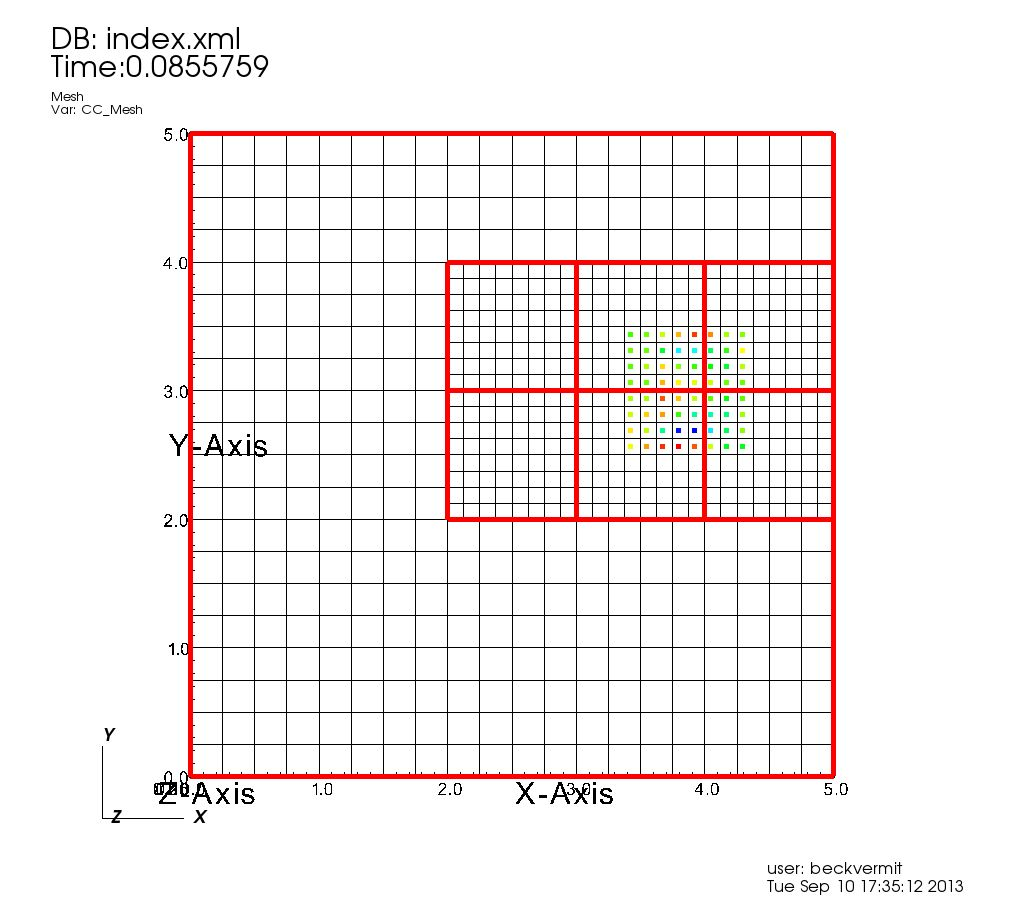
\includegraphics[trim=0cm 3cm 0cm 3cm, clip=true, width=1.\textwidth]{min-patch-size-8-8-1.jpeg}
  \caption{Advect\_2L\_MI with a minimum patch size of [8,8,1]}
  \label{fig:881}
\end{figure}

Here the black lines represent cells and the red lines represent patches with the box of multi-colored points being particles. As can be seen, there are 8 cells per patch in the x and y-direction and only one cell per patch in the z-direction (2D simulation). When we increase the minimum patch size to [20,20,1] we see:

\begin{figure}[H]
  \centering
  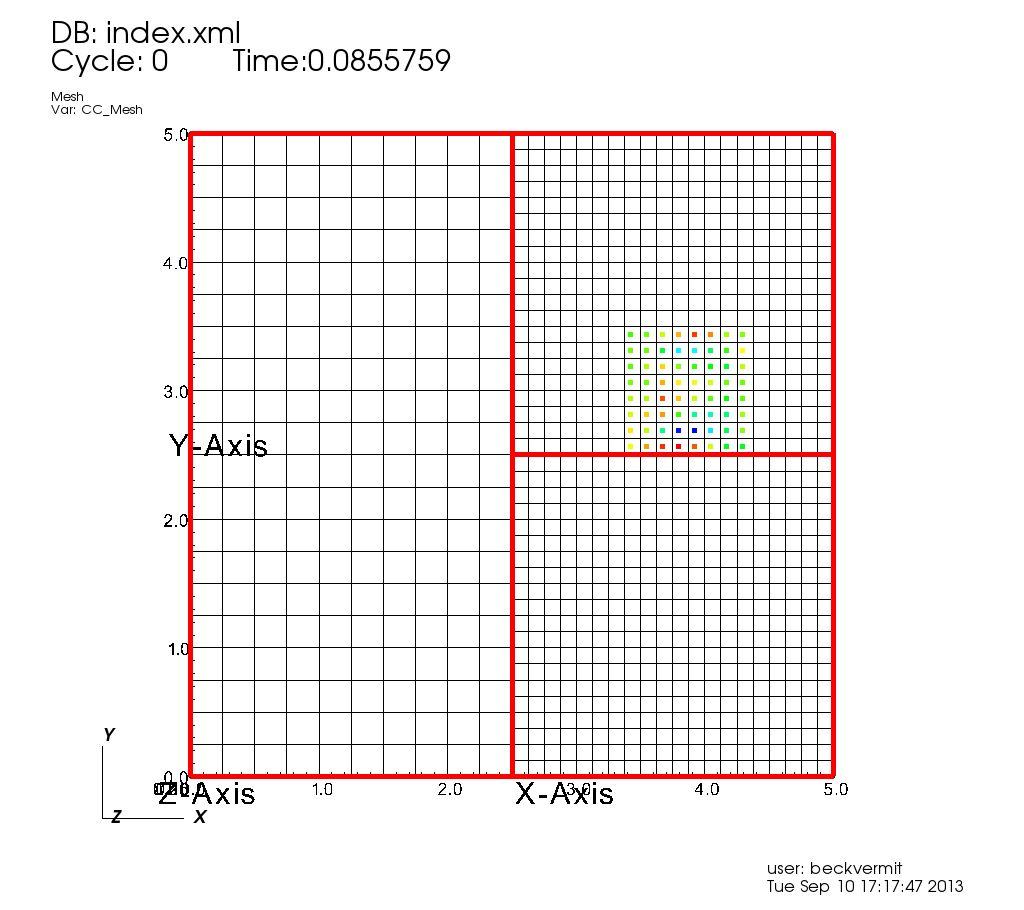
\includegraphics[trim=0cm 3cm 0cm 3cm, clip=true, width=1.\textwidth]{min_patch_size-20-20-1.jpeg}
  \caption{Advect\_2L\_MI with a minimum patch size of [20,20,1]}
  \label{}
\end{figure}

Note that now there are only 2 patches covering our finest level compared to the 6 patches covering our finest levels in figure \ref{fig:881}. This is because there is enough ``padding'' in between our refinement flags and differing levels to avoid setting up whole new patches at the most refined level. This option can be adjusted to increase or decrease the overall amount of regridding necessary with the cell\_regrid\_dilation flag.

When we decrease our minimum patch size to [4,4,1] we see:
\begin{figure}[H]
  \centering
  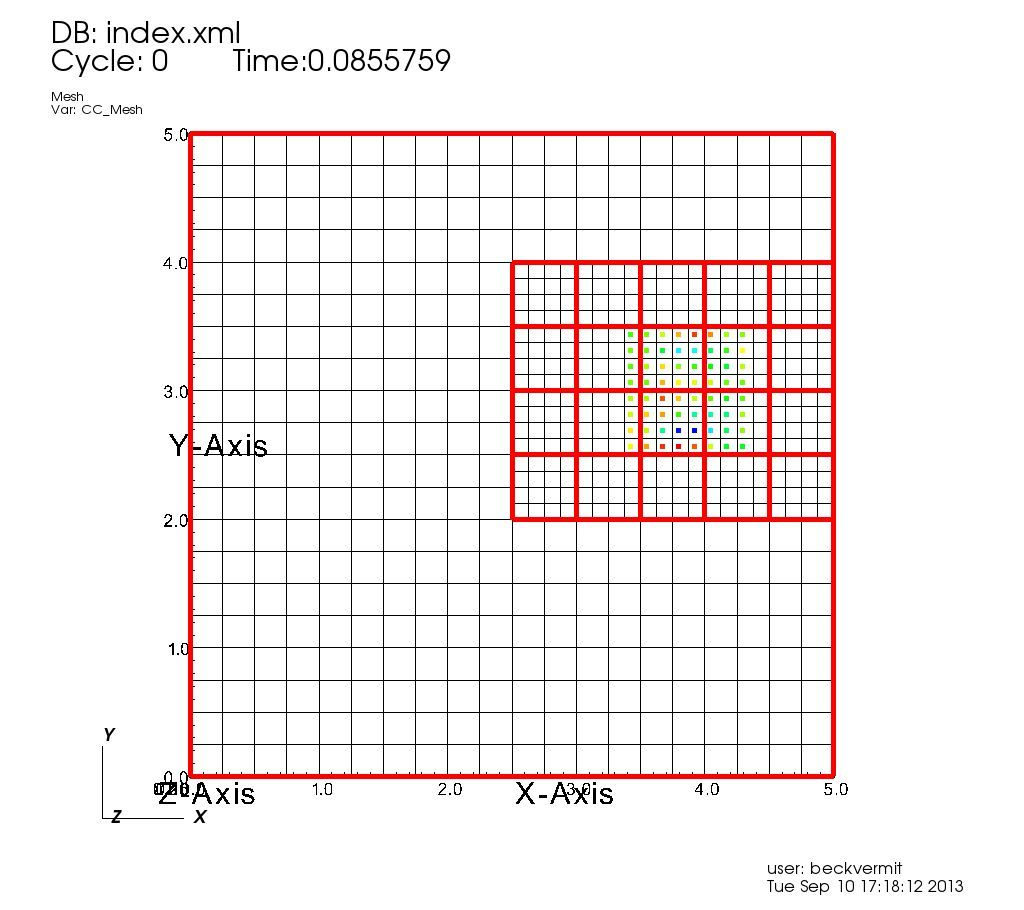
\includegraphics[trim=0cm 3cm 0cm 3cm, clip=true, width=1.\textwidth]{min_patch_size-4-4-1.jpeg}
  \caption{Advect\_2L\_MI with a minimum patch size of [4,4,1]}
  \label{fig:441}
\end{figure}

The best way to increase the ``padding'' of your simulation and therefore decrease the number of regrids required is to increase the cell\_stability\_dilation. Below we see the 2 dimensional example with a minimum patch size of [8,8,1], like figure \ref{fig:881}, but with a cell stability dilation of [10,10,1] rather than [2,2,1].

\begin{figure}[H]
  \centering
  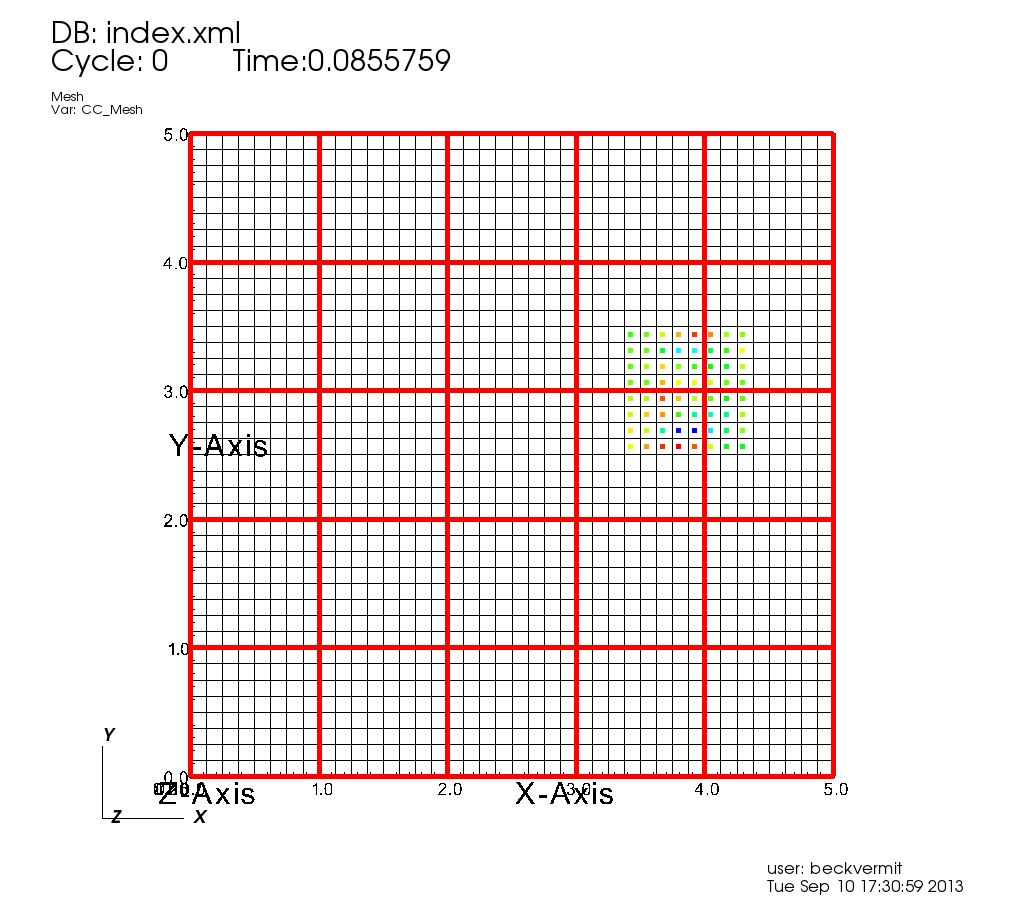
\includegraphics[trim=0cm 3cm 0cm 3cm, clip=true, width=1.\textwidth]{cell_stability_dialation-10-10-1.jpeg}
  \caption{Advect\_2L\_MI with a minimum patch size of [8,8,1] and a cell stability dilation of [10,10,1]}
  \label{fig:10101}
\end{figure}

There is a balance between cell stability dilation and computational time. If your domain is set up like figure \ref{fig:10101}, less computational time will be wasted regridding. However, it could be more economical to utilize some coarser levels in the areas that see little or no particles.


\subsection{AMR Grids}


There are two ways to run with mesh-refinement, either adaptive or
non-adaptive (static). Adaptive grids are created based on the
existence of refinement flags that are created during the
simulation. A regridder will analyze the whole domain, and, wherever there are
refinement flags, construct patches around them on a finer
level. See more on Regridding below.

\subsubsection{Regridding}


For an adaptive problem, specify the Regridder section in the input
file. The Tiled regridder works as follows:

Tiles sized according to the minimum patch size are laid across domain. Refinement flags are then used to determine which of
those tiles are in the patch set. If the number of tiles is more than
twice the target number of patches then the tile size is doubled in
the shortest dimension. If the number of tiles is less than the target
number of patches then the tile size is halved in the longest
dimension. The tile size will never get smaller than the minimum
specified tile size. This regridder produces regular patch sets that
are easy to load balance. After patches are added, data is stored on them. Then data will be
initialized for those new patches, and in the next timestep, those
patches will be included in the regridding process.

A constraint of the Regridder is that any two patches that share a boundary must be within one level of each other. See (E) and (F) below.

%At initialization time, the regridder can be executed and then the
%problem reinitialized so the problem can be initialized with all
%5max\_levels of refinement.

\begin{figure}[H]
  \centering
  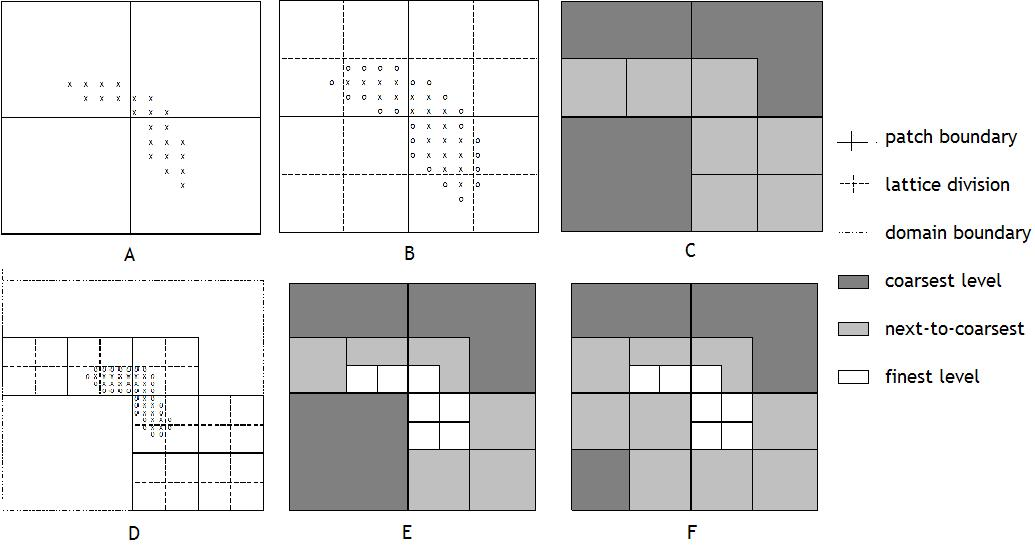
\includegraphics[width=1.\textwidth]{AMR-Regridding.jpg}
  \caption{}
  \label{}
\end{figure}

In the diagram above, image (A) show 4 coarse patches with some marked
error flags. (B) Shows the subpatches for the next level and has the
error flags dilated. (C) Shows the coarse level together with the fine
level you end up with.

(D) During the next regrid, the next level can create error flags as
well. These are some example error flags that are dilated, with the
subpatches for the next level. (E) shows the resulting level with the
other levels. However there are some patch boundaries that span more
than one level. So in (F) we must expand out the middle level to
compensate.

Note that if you define multiple levels in the input file, all but
the coarsest level will be recycled, and levels will be added where
the Regridder wants to put them.

\subsubsection{Static Grids}

Static grids can be defined by simply not including a Regridder
section in the input file. See the multiple level example in
Grid~\ref{Sec:Grid}.

\subsubsection{Ideal Patch Configuration for Good Scaling}
The patch configuration on multiple levels has been shown to greatly
effect the scalability and mean time per time step.
Here are some guidelines to follow when trying to get good scaling with multilevel AMR.
This example is for a 3 Level simulation.
\begin{itemize}
\item On Level 0 and 1 $\frac{\# cells}{patch} = 8$ \\	
	i.e. min\_patch\_size [8,8,8]
\item On finer levels (level 2)
\begin{itemize}
	\item min\_patch\_size MUST be greater than or equal to 8,8,8!! This is very important!
	\item $\frac{\# cores}{2} $ $\leq$ $\#$ patches on the finest level $\leq$ $\#$ cores
	\item The min\_patch\_size on L-2 must be divisible by the min\_patch\_size on L-1
\end{itemize}
\end{itemize}

\subsection{AMR Cycle}

Whether working with an adaptive or a static grid, AMR problems follow
the same cycle.

In short, there are 3 main AMR operations
\begin{itemize}

\item Coarsen - This occurs after each execution of a finer level, if
  the time of the finer level lines up with the time of the coarser
  level (see the ``W-cycle'' diagram). Its data are coarsened to the
  coarser level so that the coarse level has a representation of the
  data at the finest resolution. Also as part of this operation is the
  ``reflux'' operations, which to makes the fluxes across the face of
  the coarse-fine boundary consistent across levels.
\item Refine the coarse-fine interface - This occurs after the
  execution of each level and after an associated coarsen (if
  applicable). The cells of the boundary of the finer level are
  interpolated with the nearest cells on the coarser level (so the
  finer level stays in sync with the coarser levels).
\item Refine - This occurs for new patches created by the regrid
  operation. Variables that are necessary will be created on those
  patches by interpolation from the coarser level.
\end{itemize}

After an entire cycle, then we check to see if we need to regrid. If the flags haven't changed such that patches would form, the grid will remain the same.

In short, these diagrams may be useful:

``W-cycle'' (time refinement ratio of 2)

\begin{figure}[h]
  \centering
  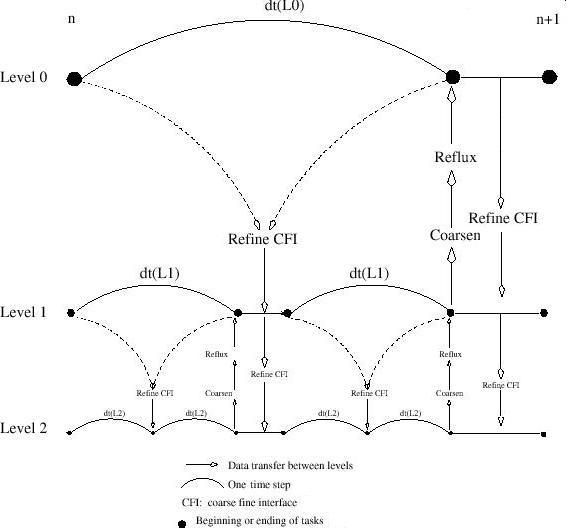
\includegraphics[width=.75\textwidth]{AMR-Cycle-W.jpg}
  \caption{}
  \label{}
\end{figure}

``Lockstep cycle''

\begin{figure}[h]
  \centering
  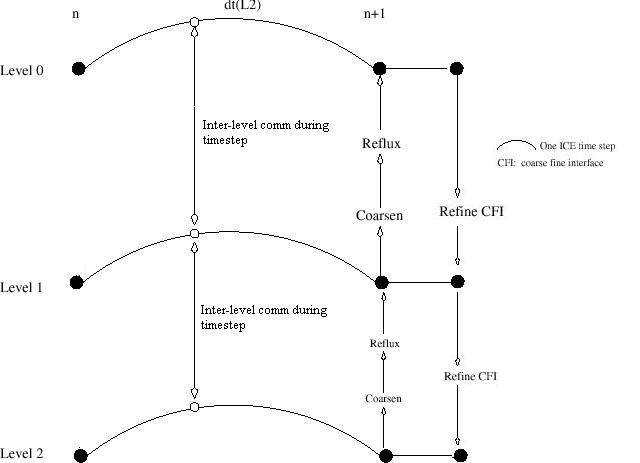
\includegraphics[width=.75\textwidth]{AMR-Cycle-Lock.jpg}
  \caption{}
  \label{}
\end{figure}

\section{Regridder}

The regridder creates a multilevel grid from the refinement flags.
Each level will completely cover the refinement flags from the coarser
level.  The primary regridder used in Uintah is the \TT{Tiled} regridder.
The tiled regridder creates a set of evenly sized tiles across the domain
that will become patches if refinement is required in the tiles region.

The following is an example of this regridder.

\begin{Verbatim}[fontsize=\footnotesize]
<Regridder type="Tiled">   
    <max_levels>2</max_levels>
    <cell_refinement_ratio> [[2,2,1]] </cell_refinement_ratio>
    <cell_stability_dilation> [2,2,0] </cell_stability_dilation>
    <min_boundary_cells> [1,1,0] </min_boundary_cells>
    <min_patch_size>  [[8,8,1]] </min_patch_size>
</Regridder>
\end{Verbatim}

The \TT{max\_levels} tag specifies the maximum number of levels
to be created.  The \TT{cell\_refinement\_ratio} tag specifies the 
refinement ratio between the levels.  This can be specified on a per 
level basis as follows:

\begin{Verbatim}[fontsize=\footnotesize]
    <cell_refinement_ratio> [[2,2,1],[4,4,1]] </cell_refinement_ratio>
\end{Verbatim}

The \TT{cell\_stability\_dilation} tag specifies how many cells around
the refinement flags are also guaranteed to be refined.  The
\TT{min\_boundary\_cells} tag specifies the size of the boundary layers. 
The size of the tiles is specified using the \TT{min\_patch\_size} tag
and can also be specified on a per level basis.

%
%__________________________________
\section{Dynamic Load Balancing} \label{loadbalancer}

Uintah has a couple of load balancing options which may be useful for increasing performance by decreasing
the load imbalance.  The following describes the loadbalancer section of an input file and what effects
it has on the load balancer.  

If no load balancer is specified then a simple load balancing method which assigns an equal number of patches
to processors. This is not ideal in most cases and should be avoided.

\subsection{Input File Specs}
\begin{Verbatim}[fontsize=\footnotesize]
   <LoadBalancer type="DLB"> 
        <!-- DLB specific flags -->
        <costAlgorithm>ModelLS</costAlgorithm>
        <hasParticles>true</hasParticles>

        <!-- DLB/PLB flags -->
        <timestepInterval>25</timestepInterval>
        <gainThreshold>0.15</gainThreshold>
        <outputNthProc>1</outputNthProc>
        <doSpaceCurve>true</doSpaceCurve>

   </LoadBalancer>
\end{Verbatim}

There are two main load balancers used in Uintah.  The first is the DLB load balancer.
This is a robust load balancer that is good for many problems.  In addition,
this load balancer can utilize profiling in order to tune itself during the runtime
in order to achieve better results.  

To use this load balancer the user must specify the type as "DLB".  It is also suggested
that the user specify a costAlgorithm which can be "Model", "ModelLS", "Memory", or
"Kalman" with the default being "ModelLS".  If "hasParticles" is set to true then
these cost algorithms will take the number of particles into account when determining
the cost.

This algorithm first orders the patches linearly.  If doSpaceCurve is set to true
then this ordering is done according to a Hilbert Space-Filling curve, which will
likely provide better clusterings.  Once the patches are ordered linearly, costs
are assigned to each patch and the patches are distributed onto processors so that
the costs on each processor are even.  

The PLB load balancer is an alterantive to the DLB load balancer which is
likely more efficent for particle based calculations.  This load balancer
divides the patches into two sets (cell dominate and particle domintate), 
which is determined using the particleCost and cellCost parameters.
The particle dominate patches are then assigned to processors while trying
to equalize the number of particles on each processor.  Finally the 
cell dominate patches are assigned to patches in order to equalize the number
of cells while accounting for the number of cells already assigned during 
the particle assignment phase.  This method can also utilize a space-filling
curve.  

The following list describes other flags utilized by these load balancers:
\begin{itemize}
  \item timestepInterval - how many timesteps must pass before reevaluating the load balance.  
  \item gainThreshold - the predicted percent improvement that is required to reload balance.  
  \item outputNthProc - output data on only every Nth processor (experimental). 
\end{itemize}



%__________________________________
\section{UDA}

%\subsection{UDA Directory Structure}

The UDA is a file/directory structure used to save Uintah simulation
data.  For the most part, the user need not concern himself with the
UDA layout, but it is a good idea to have a general feeling for how
the data is stored on disk.

%\subsubsection{UDA Naming}

Every time a simulation (sus) is run, a new UDA is created.  Sus uses
the $<$filebase$>$ tag in the simulation input file to name the UDA
directory (appending a version number).  If an UDA of that name
already exists, the next version number is used.  Additionally, a
symbolic link named ``disks.uda'' (is updated to and) will point to
the newest version of this simulations UDA.  Eg:

\begin{Verbatim}[fontsize=\footnotesize]
disks.uda.000
disks.uda.001
disks.uda.001 <- disks.uda
\end{Verbatim}

%\subsubsection{UDA Files}

Each UDA consists of a number of top level files, a checkpoints
subdirectory, and subdirectories for each saved timestep.  These files
include:

\begin{itemize}

\item \tt.dat \normalfont files contain global information about the
  simulation (each line in the .dat files contains: simulation\_time
  value).
\item \tt checkpoints \normalfont directory contains a limited
  number of time step data subdirectories that contain a complete
  snapshot of the simulation (allowing for the simulation to be
  restarted from that time).
\item \tt input.xml \normalfont contains the original problem
  specification (the .ups file).
\item \tt index.xml \normalfont contains information on the actual
  simulation run.
\item \tt t0000\# \normalfont contains data saved for that specific
  time step.  The data saved is specified in .ups file and may be a
  very limited subset of the full simulation data.

\end{itemize}

The 'validateUda' script (src/Packages/Uintah/scripts/) can be used to
test the integrity of a UDA directory. It does not interogate the data
for 'correctness', but it performs 5 basic tests on each uda:

\begin{Verbatim}
Usage validateUda  <udas>
Test 0:  Does index.xml exist?                                        true or false
Test 1:  Does each timestep in index.xml exist?                       true or false
Test 2:  Do all timesteps.xml files exist?                            true or false
Test 3:  Do all the level directories exist:                          true or false
Test 4:  Do all of the pxxxx.xml files exist and have size >0:        true or false
Test 5:  Do all of the pxxxx.data files exist and have size > 0:      true or false
\end{Verbatim}

If any of the tests fail then the corrupt output timestep should be removed from the index.xml file.


See Section~\ref{Sec:DataArchiver} for a description of how to specify
what data are saved and how frequently.

% The following seems not that useful to me.  JG
%Example UDA file list:

%CenterOfMassPosition.dat
%CenterOfMassVelocity.dat
%KineticEnergy.dat
%StrainEnergy.dat
%TotalMass.dat
%checkpoints
%index.xml
%input.xml
%t00001
%t00057

%\subsection{Known Issues}

%Occasionally, due (most likely) to file system issues on large
%clusters, some of the files in the UDA have been found to be corrupted
%or nonexistent.  (There is error checking in the code to try to
%prevent this.  We believe that either the OS/File system is
%incorreclty returning error codes, or, more likely, that the files are
%corrupted (due to file system issues) after the simulation is done.

%\subsection{Restarting}

%The sus executable provides a mechanism for checkpointing the code and
%then restarting the ongoing simulation from a given checkpoint.



%__________________________________
\chapter{Visualization tools -- VisIt}

Visualization of Uintah data is currently possible using any of two
software packages.  These are SCIRun and VisIt.  Of these, SCIRun is
no longer supported, although legacy versions will continue to work.
The VisIt package from LLNL is general purpose visualization software
that offers all of the usual capabilities for rendering scientific
data.  It is still developed and maintained by LLNL staff, and its
interface to Uintah data is supported by the Uintah team. 

%Manta offers volume rendering and particle visualization based on
%parallel (shared memory) ray tracing techniques.  While the
%capabilities of Manta are more limited, it is a fast way to
%interactively interrogate reasonably large datasets, provided the user
%has access to a reasonable shared memory resource, (e.g. an 8 core
%desktop system).


\section{Reading Uintah Data Archives}

\begin{wrapfigure}{r}{.50\textwidth}
  \vspace{-30pt}
  \begin{center}
    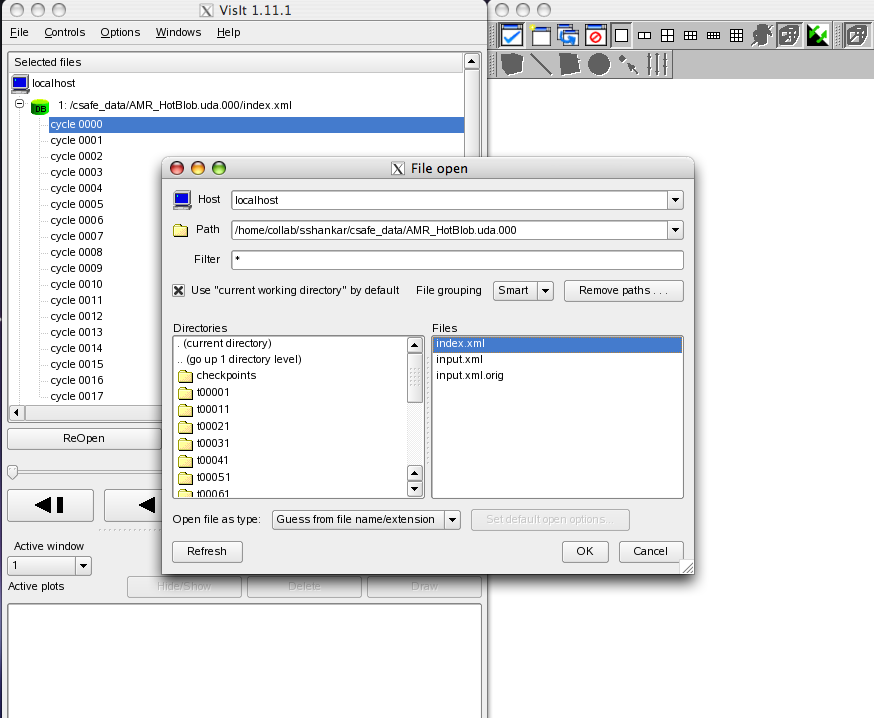
\includegraphics[width=.3\textwidth]{VisItFileOpen.png}
  \end{center}
  \vspace{-20pt}
  \caption{Opening an UDA with VisIt}
  \vspace{-10pt}
  \label{VisItFileOpen}
\end{wrapfigure}


Once you have installed VisIt and the UDA reader plugin, you can
launch VisIt and start visualizing UDA's. To open a UDA, select \tt
Open File \normalfont from the \tt File \normalfont menu. Browse into
the UDA you want to load and select the \tt index.xml \normalfont
file. Then hit on \tt OK \normalfont and a list of timesteps should
now appear on the gui. Figure~\ref{VisItFileOpen} illustrates this
process.


\section{Plots}

\begin{wrapfigure}{r}{.50\textwidth}
  \vspace{-65pt}
  \center
  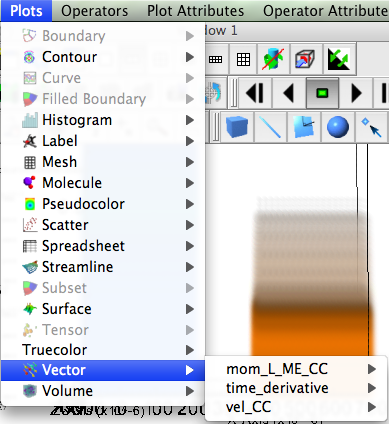
\includegraphics[width=.3\textwidth]{VisItPlots.png}
  \vspace{-10pt}
  \caption{Various plots in VisIt}
  \vspace{-50pt}
  \label{VisItPlots}
\end{wrapfigure}


VisIt displays data as plots. A plot might render a specific variable
or it might render the structure of the mesh. Figure~\ref{VisItPlots}
illustrates this.


Note that VisIt attempts to analyze the variables and associate them
with the appropriate plots. As shown in Figure~\ref{VisItPlots}, only
vector variables are available for the vector plot. The most commonly
used plots for visualizing UDA's are Pseudocolor, Volume and the
Vector plot. The Subset plot can be used to visualize the structure of
patches in an AMR dataset.
%The Mesh plot can be used to display the mesh structure.

\begin{wrapfigure}{r}{.50\textwidth}
  \vspace{-20pt}
  \center
  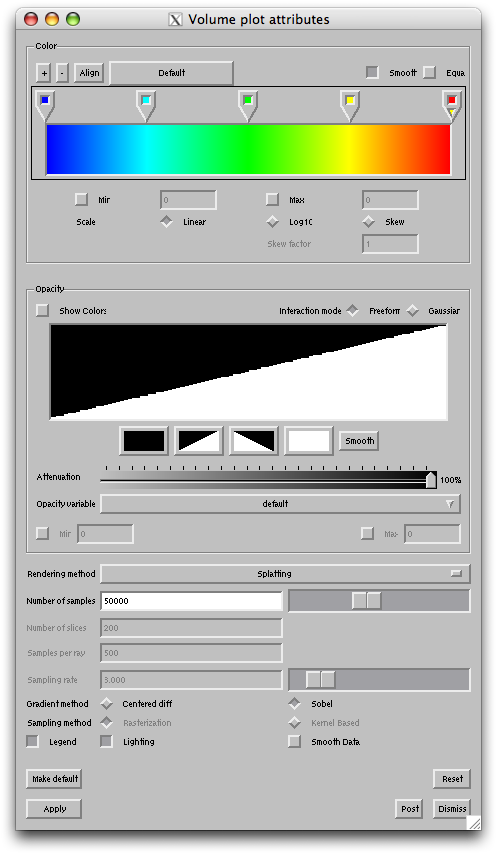
\includegraphics[width=.30\textwidth]{VisItVolumeAtts.png}
  \vspace{-10pt}
  \caption{Volume plot attributes in VisIt}
  \vspace{-40pt}
  \label{VisItVolumeAtts}
\end{wrapfigure}


Once you have a plot, you change plot attributes by clicking on the
PlotAtts menu and selecting the plot of you choice. Alternatively, you
may double click on the plot itself in Active plots window. For
example, if you have a Volume plot and you want to change its
attributes, the window shown in Figure~\ref{VisItVolumeAtts} pops up.



As seen in Figure~\ref{VisItVolumeAtts}, you can change the color map,
opacity curve, rendering method, no. of samples, lighting options,
etc. in this window.



\section{Operators}

\begin{wrapfigure}{r}{.50\textwidth}
  \vspace{-20pt}
  \center
  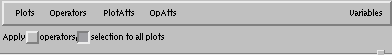
\includegraphics[width=.3\textwidth]{VisItApplyOperators.png}
  \vspace{-10pt}
  \caption{Unchecking "selection to all plots"}
  \vspace{-10pt}
  \label{VisItApplyOperators}
\end{wrapfigure}


A wide variety of operators can be applied to the plots, as mentioned
earlier. These modify the incoming datasets in some way (eg., a slice
formats a 3D dataset into a 2D slice), which can then be
plotted. However, you will first need to select a plot and then only
you can apply an operator to it (though the order of operation is
opposite). An important thing to keep in mind is that when you select
an operator, by default it gets applied to all the plots in the Active
plots window. You will need to uncheck the Apply operators checkbox,
in case you just want to apply the operator to a single plot as shown
in Figure~\ref{VisItApplyOperators}.


The entire list of operators that VisIt supports can be seen by
clicking on the Operators menu. Also, once you have applied an
operator, you can change its attributes by clicking on the OpAtts menu
and then clicking on the desired operator.
Figures~\ref{VisItSelectPlot} and~\ref{VisItSelectOperator} illustrate
how you can apply a Slice operator to a Pseudocolor plot and then
change the operator attributes.  First, apply the Pseudocolor plot to
a desired variable, and then select the Slice operator from the
Operators menu.

% \begin{wrapfigure}{r}{.50\textwidth}
%   \vspace{-10pt}
%   \center
%   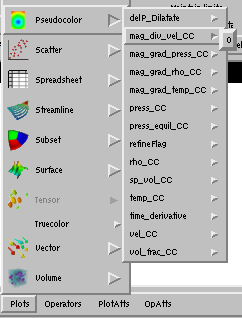
\includegraphics[width=.3\textwidth]{VisItSelectPlot.png}
%   \caption{Applying the Pseudocolor plot to a variable}
%   \vspace{10pt}
%   \label{VisItSelectPlot}
% \end{wrapfigure}


% \begin{wrapfigure}{r}{.50\textwidth}
%   \center
%   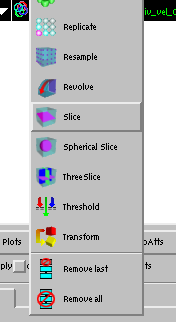
\includegraphics[width=.3\textwidth]{VisItSelectOperator.png}
%   \caption{Applying an operator to a plot}
%   \label{VisItSelectOperator}
% \end{wrapfigure}


\begin{figure}
  \vspace{-100pt}
  \centering 
  \subfloat[Applying the Pseudocolor plot to a variable]{\label{VisItSelectPlot}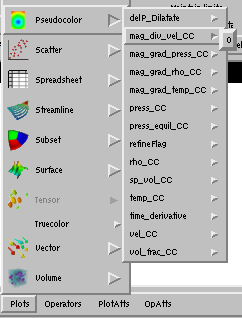
\includegraphics[width=0.3\textwidth]{VisItSelectPlot.png}}
  \hspace{50pts}
  \subfloat[Applying an operator to a plot]{\label{VisItSelectOperator}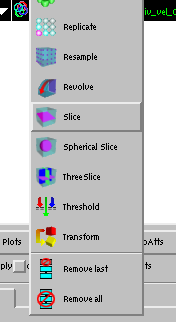
\includegraphics[width=0.3\textwidth]{VisItSelectOperator.png}}
  \caption{}
  \label{}
\end{figure}


\begin{figure}
  \centering
  \vspace{-20pt}
  \subfloat[Ordering of an operator and a plot]{\label{VisItOrderOperator}
  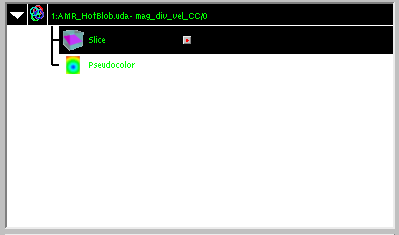
\includegraphics[width=.3\textwidth]{VisItOrderOperator.png}}
  \hspace{50pt}
  \subfloat[Slice plot attributes in VisIt]{\label{VisItSliceAtts}
  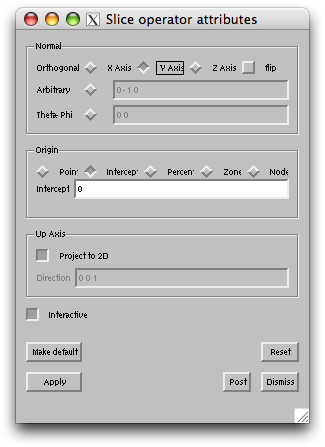
\includegraphics[width=.3\textwidth]{VisItSliceAtts.png}}
  \caption{}
  \label{}
\end{figure}

% \begin{wrapfigure}{R}{.50\textwidth}
%   \center
%   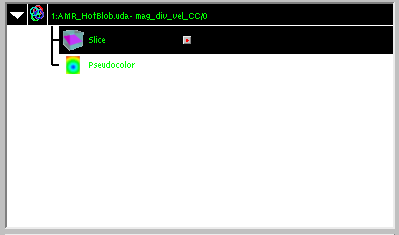
\includegraphics[width=.3\textwidth]{VisItOrderOperator.png}
%   \caption{Ordering of an operator and a plot}
%   \label{VisItSliceAtts}
% \end{wrapfigure}

At this point in time, you should have an ordering similar to that in
Figure~\ref{VisItOrderOperator}.  Once you have this order, select
Slice from the OpAtts menu. This will pop up the Slice operator
attributes window, as shown in Figure~\ref{VisItSliceAtts}.

% \begin{wrapfigure}{r}{.50\textwidth}
%   \center
%   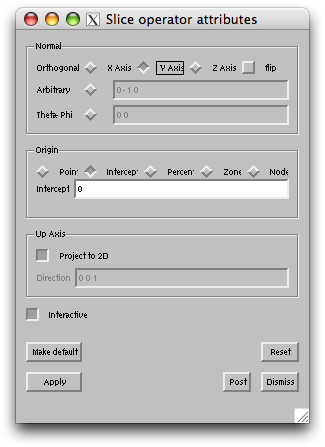
\includegraphics[width=.4\textwidth]{VisItSliceAtts.png}
%   \caption{Slice plot attributes in VisIt}
%   \label{VisItSliceAtts}
% \end{wrapfigure}

You can now play up with the various attributes (eg., selecting normal
plane) to obtain the desired visualization. The checkbox "Project to
2D" should be unchecked is you want to have the slice in 3D space.

\section{Vectors}

\begin{wrapfigure}{r}{.50\textwidth}
  \center
  \vspace{-40pts}
  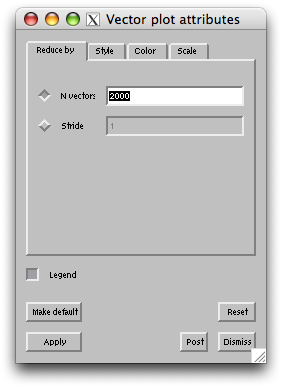
\includegraphics[width=.48\linewidth]{VisItVectorNumber.png}
  \caption{Increasing the number of Vectors}
  \vspace{-20pts}
  \label{VisItVectorNumber}
\end{wrapfigure}


By default, VisIt reduces the number of vectors plotted (to 400) and
this needs to be manually changed to the original number or something
greater, only if required.  This can be accomplished by changing the
attributes of the Vector plot. In Figure~\ref{VisItVectorNumber}, the
number of vectors has been increased to 2000.


\begin{wrapfigure}{r}{.50\textwidth}
  \center
  \vspace{-50pts}
  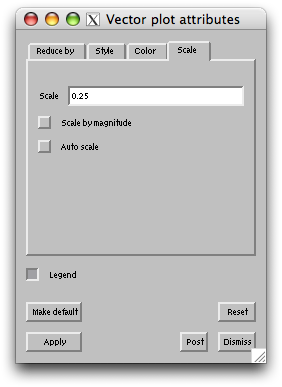
\includegraphics[width=.3\textwidth]{VisItVectorScale.png}
  \caption{Increasing the scale of Vectors}
  \vspace{-30pts}
  \label{VisItVectorScale}
\end{wrapfigure}


Also if you would like all the vectors to be visible, you would need
to switch off both the options, \tt Scale by magnitude \normalfont and
\tt Auto scale \normalfont under the Scale tab in the same window as
shown in figure~\ref{VisItVectorScale} describes this.


\section{AMR datasets}



AMR datasets are read the same way as single level datasets. Once you
have it read, you can apply an plot/ operator on it. Since the dataset
is organized as levels and patches, you now have the flexibility of
visualizing each of them independently or as in a group. To achieve
this (assuming that you have already selected a plot), click on the
Subset button either on the Active Plots window in the gui or on the
same option in the Controls menu. This is illustrated in
Figures~\ref{VisItSubsetIcon} and ~\ref{VisItSubsetWin}.

% \begin{wrapfigure}{r}{100mm}
%   \center
%   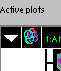
\includegraphics[width=.5\linewidth]{VisItSubsetIcon.png}
%   \caption{Clicking on this icon pops up the Subset window}
%   \label{VisItSubsetIcon}
% \end{wrapfigure}

% \begin{wrapfigure}{r}{100mm}
%   \center
%   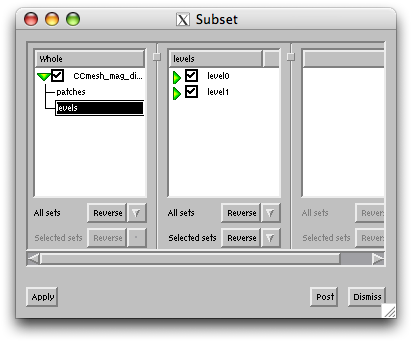
\includegraphics[width=.5\linewidth]{VisItSubsetWin.png}
%   \caption{The Subset window in VisIt}
%   \label{VisItSubsetWin}
% \end{wrapfigure}

\begin{figure}
  \centering
  \vspace{-80pt}
  \subfloat[Clicking on this icon pops up the Subset window]{\label{VisItSubsetIcon}
  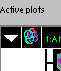
\includegraphics[width=.3\linewidth]{VisItSubsetIcon.png}}
  \hspace{50pt}
  \subfloat[The Subset window in VisIt]{\label{VisItSubsetWin}
  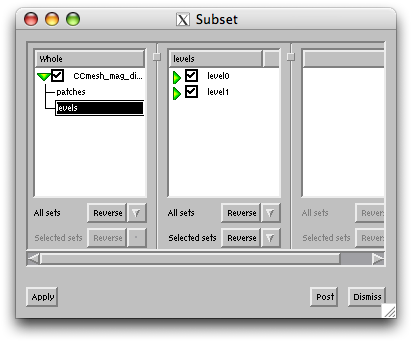
\includegraphics[width=.3\linewidth]{VisItSubsetWin.png}}
  \caption{}
  \vspace{-10pt}
  \label{}
\end{figure}


\section{Examples}

\subsection{Volume visualization}

\begin{enumerate}

\item Read in the uda by selecting the index.xml file. A list of
  timesteps should now appear on the gui.

% \begin{wrapfigure}{r}{.50\textwidth}
%   \center
%   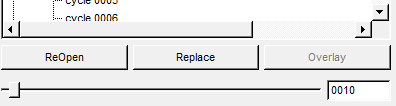
\includegraphics[width=.3\textwidth]{VisItTimestepBox.png}
%   \caption{The window on the gui lists all the timesteps}
%   \label{VisItTimestepBox}
% \end{wrapfigure}


\item The first timestep (cycle 0000) should be preselected. In case you
are interested in plotting a different timestep, just double click on
it. Alternatively you can type it in the small rectangular box
(Figure~\ref{VisItTimestepBox}), just below the list of
timesteps. This can also be done at a later period in time, when you
are done plotting the variable associated with a specific timestep and
want to traverse through the others.


\item Next we select a variable to plotted. We click on the Plots
  menu, select the Volume plot and then select the variable tempIN as
  shown in the Figure~\ref{VisItVolumeTempINATK08}. The number '1'
  refers to the material associated with the variable.

% \begin{wrapfigure}{r}{.50\textwidth}
%   \center
%   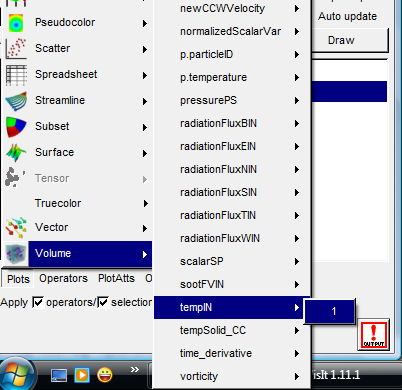
\includegraphics[width=.3\textwidth]{VisItVolumeTempINATK08.png}
%   \caption{Selecting a volume plot and an associated variable/ material}
%   \label{VisItVolumeTempINATK08}
% \end{wrapfigure}

\item The variable tempIN/1 now appears on the Active plots window
  (Figure~\ref{VisItDrawTempINATK08}). Select the variable and click
  Draw.

\begin{figure}[h]
  \centering
  \vspace{-10pt}
  \subfloat[The window on the gui lists all the timesteps]{\label{VisItTimestepBox}
  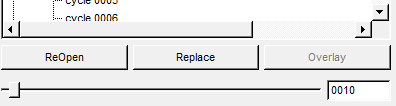
\includegraphics[width=.3\textwidth]{VisItTimestepBox.png}}
  \hspace{10pt}
  \subfloat[Selecting a volume plot and an associated variable/ material]{\label{VisItVolumeTempINATK08}
  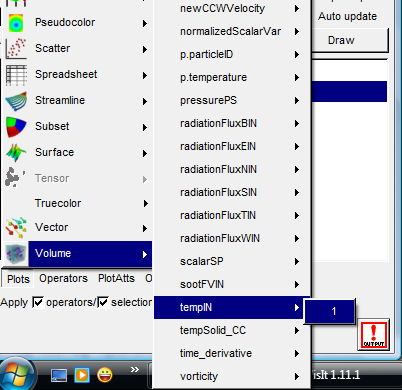
\includegraphics[width=.3\textwidth]{VisItVolumeTempINATK08.png}}
  \hspace{10pt}
  \subfloat[The list of plots in the Active plots window]{\label{VisItDrawTempINATK08}
  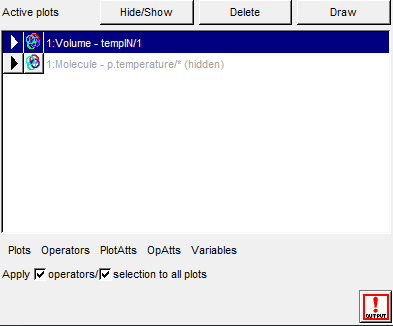
\includegraphics[width=.3\textwidth]{VisItDrawTempINATK08.png}}
  \caption{}
  \vspace{-10pt}
  \label{}
\end{figure}




% \begin{wrapfigure}{r}{.50\textwidth}
%   \center
%   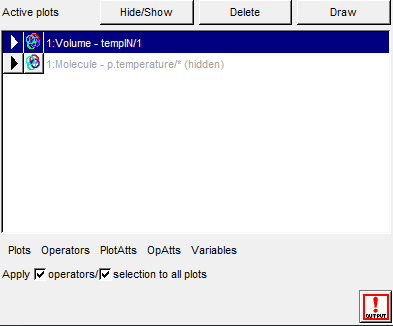
\includegraphics[width=.4\textwidth]{VisItDrawTempINATK08.png}
%   \caption{The list of plots in the Active plots window}
%   \label{VisItDrawTempINATK08}
% \end{wrapfigure}

\item A visualization now appears on the Viewer window, as shown in
  Figure~\ref{VisItVolumeTempINATK08Viewer}. You can interact with the
  visualization in terms of rotating it (holding the left mouse button
  and dragging it), zooming in/ out (scrolling the roller on the mouse
  and/ or selecting the magnifier at the top of the Viewer window)
  etc.



% \begin{wrapfigure}{r}{.50\textwidth}
%   \center
%   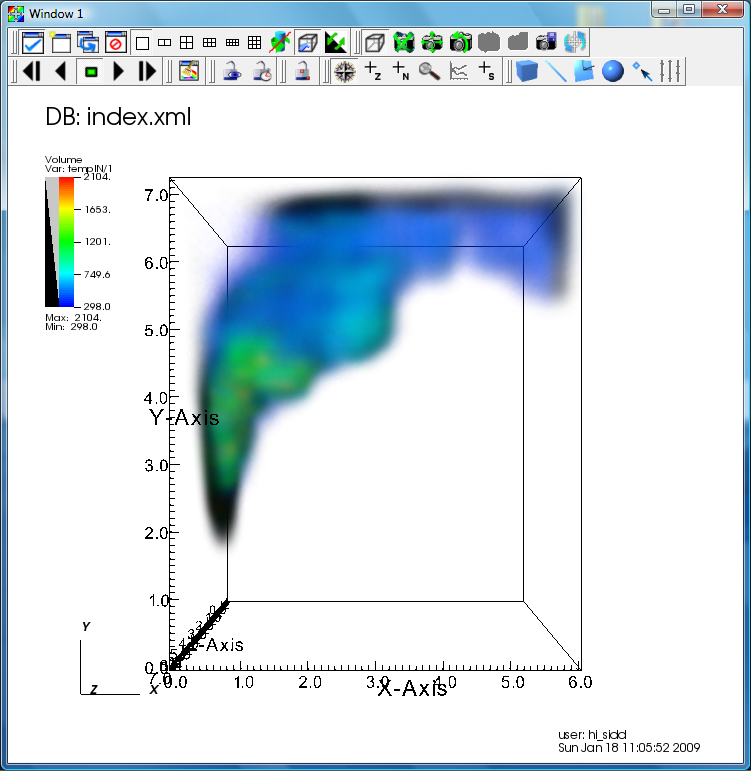
\includegraphics[width=.4\textwidth]{VisItVolumeTempINATK08Viewer.png}
%   \caption{Visualization of a volume on the viewer window}
%   \label{VisItVolumeTempINATK08Viewer}
% \end{wrapfigure}

\item Once you have this basic volume visualization, you can change
  its attributes by double clicking on the Volume - tempIN/1 plot in
  the Active plots window. This pops up the Volume plot attributes
  window (Figure~\ref{VisItVolumeAttributes1} and
  figure~\ref{VisItVolumeAttributes2}).

% \begin{wrapfigure}{r}{.50\textwidth}
%   \center
%   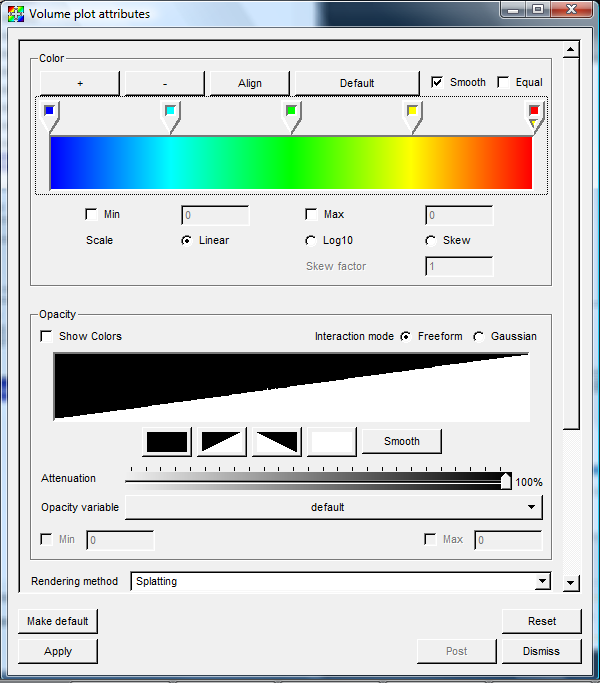
\includegraphics[width=.4\textwidth]{VisItVolumeAttributes1.png}
%   \caption{Volume visualization attributes window}
%   \label{VisItVolumeAttributes1}
% \end{wrapfigure}

% \begin{wrapfigure}{r}{.50\textwidth}
%   \center
%   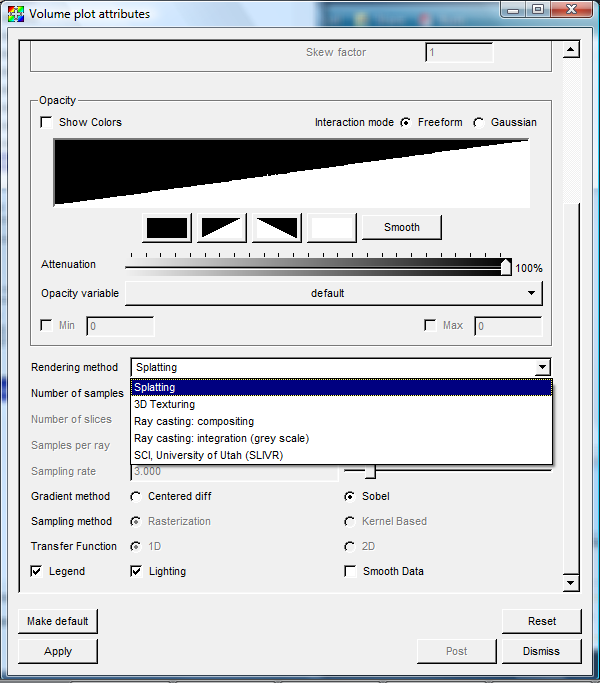
\includegraphics[width=.4\textwidth]{VisItVolumeAttributes2.png}
%   \caption{Volume visualization attributes window}
%   \label{VisItVolumeAttributes2}
% \end{wrapfigure}
\end{enumerate}


\begin{figure}[h]
  \centering
  \vspace{-10pt}
  \subfloat[Visualization of a volume on the viewer window]{\label{VisItVolumeTempINATK08Viewer}
  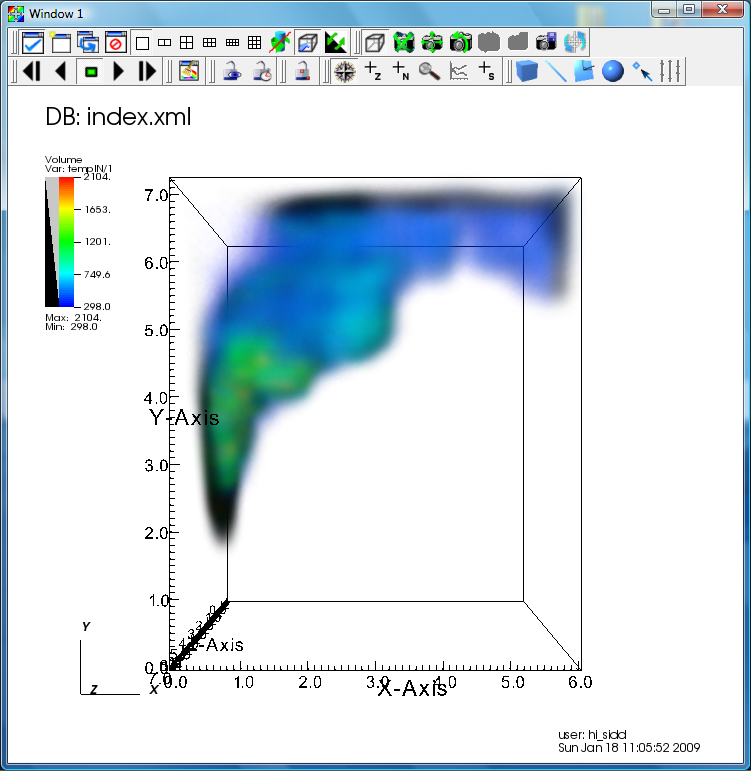
\includegraphics[width=.3\textwidth]{VisItVolumeTempINATK08Viewer.png}}
  \hspace{10pt}
  \subfloat[Volume visualization attributes window]{\label{VisItVolumeAttributes1}
  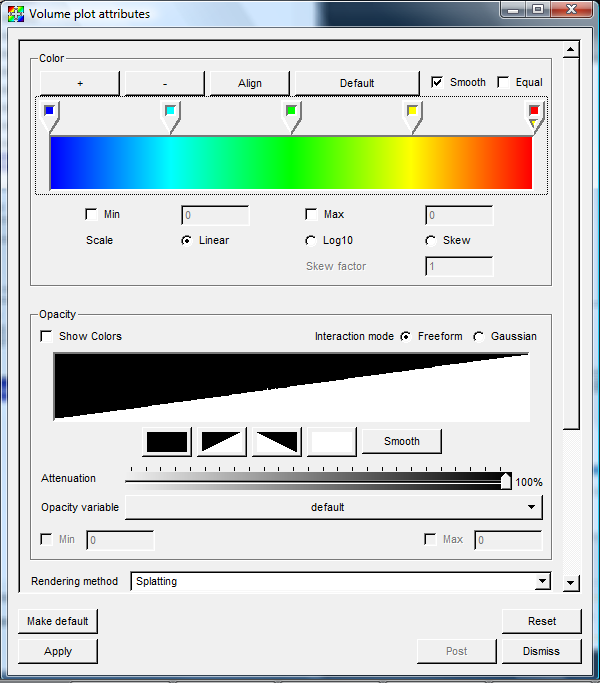
\includegraphics[width=.3\textwidth]{VisItVolumeAttributes1.png}}
  \hspace{10pt}
  \subfloat[Volume visualization attributes window]{\label{VisItVolumeAttributes2}
  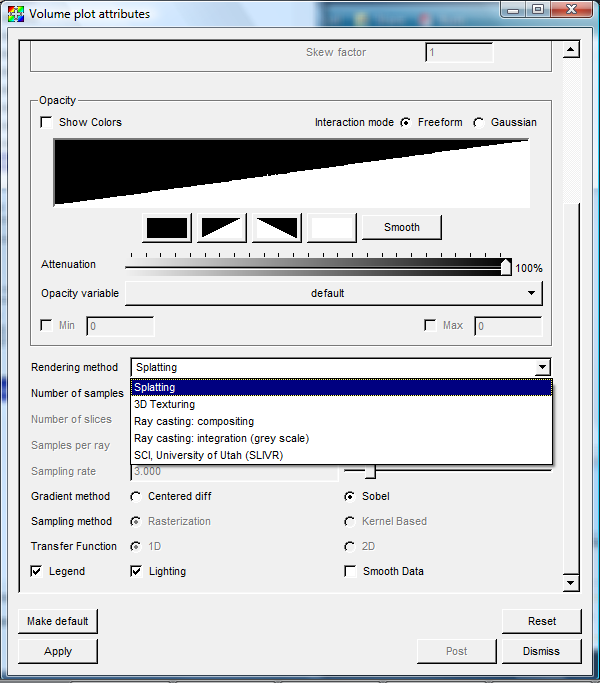
\includegraphics[width=.3\textwidth]{VisItVolumeAttributes2.png}}
  \caption{}
  \vspace{-10pt}
  \label{}
\end{figure}

The tab Color specifies the color table and the various options
associated with it. The user can add/ remove control points by
clicking on the + and - buttons. These can then be equally spaced by
pressing the Align button.

A different color table can be selected by clicking on the Default
button and then selecting an appropriate color table. The color(s)
associated with the control points can be changed by right-clicking on
the them and then selecting an appropriate color.

The user also has the option of specifying a Min and Max on the scalar
value range by checking on the associated box(s) and entering in the
values.

\begin{wrapfigure}{r}{.5\textwidth}
  \center
  \vspace{-20pt}
  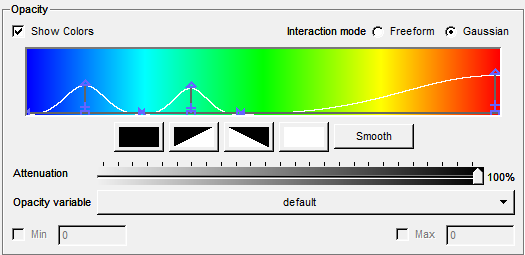
\includegraphics[width=.4\textwidth]{VisItTransferFunction.png}
  \caption{The opacity transfer function in the attributes window}
  \label{VisItTransferFunction}
\end{wrapfigure}

The second tab Opacity lets you specify a transfer function for the
color table. Clicking on the check box Show Colors copies the colors
from the color table onto this graph. Selecting the Interaction Mode
as Gaussian lets you draw curves and specify a more accurate color
table (Figure~\ref{VisItTransferFunction}).

You can add in as many curves on the graph by clicking on the left
mouse button and then placing them accordingly. To delete an unwanted
curve, just right click on it.

After specifying an opacity transfer function, one can select an
appropriate rendering method, Splatting being the default. The related
fields thereafter become active/ inactive as and when different
rendering methods are selected.

\subsection{Particle visualization}

\begin{enumerate}

\item To add particles, we select the Molecule plot and then click on
  the variable p.temperature as shown in the
  Figure~\ref{VisItMoleculePTempATK08}. The asterisk '*' refers to all
  the materials associated with the variable.

% \begin{wrapfigure}{r}{.5\textwidth}
%   \center
%   \vspace{-30pt}
%   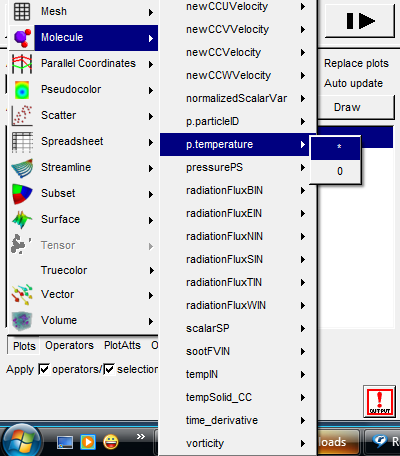
\includegraphics[width=.4\textwidth]{VisItMoleculePTempATK08.png}
%   \caption{Selecting a molecule plot and an associated variable/ material}
%   \label{VisItMoleculePTempATK08}
% \end{wrapfigure}

\item The variable p.temperature/* now appears on the Active plots
  list. Select the variable and hit Draw. A container in the form of
  particles now appears on the Viewer window.

\item Now double click on the variable name in Active plots list. This
  brings up the Molecule plot attributes window as shown in
  Figure~\ref{VisItMoleculeAttributesPTemp1}.

\end{enumerate}


\begin{figure}[h]
  \centering
  \vspace{-10pt}
 \subfloat[Selecting a molecule plot and an associated variable/ material]{\label{VisItMoleculePTempATK08}
 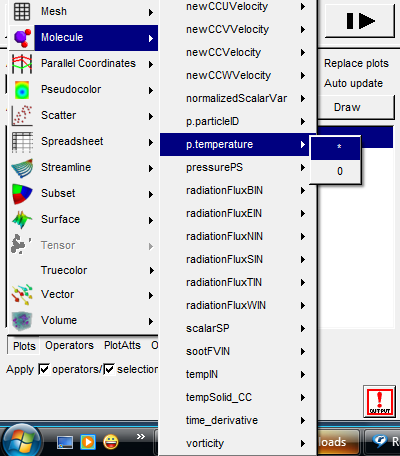
\includegraphics[width=.3\textwidth]{VisItMoleculePTempATK08.png}}
  \hspace{10pt}
 \subfloat[Selecting a molecule plot and an associated variable/ material]{\label{VisItMoleculeAttributesPTemp1}
 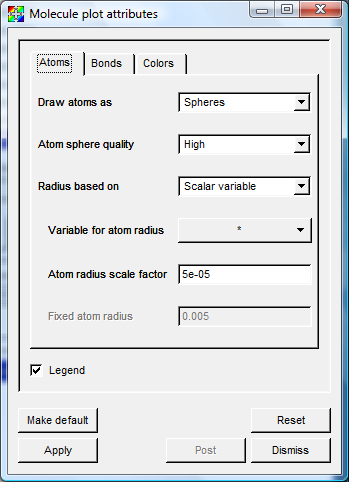
\includegraphics[width=.3\textwidth]{VisItMoleculeAttributesPTemp1.png}}
 \hspace{10pt}
 \subfloat[Selecting a molecule plot and an associated variable/ material]{\label{VisItMoleculePTtempViewer}
 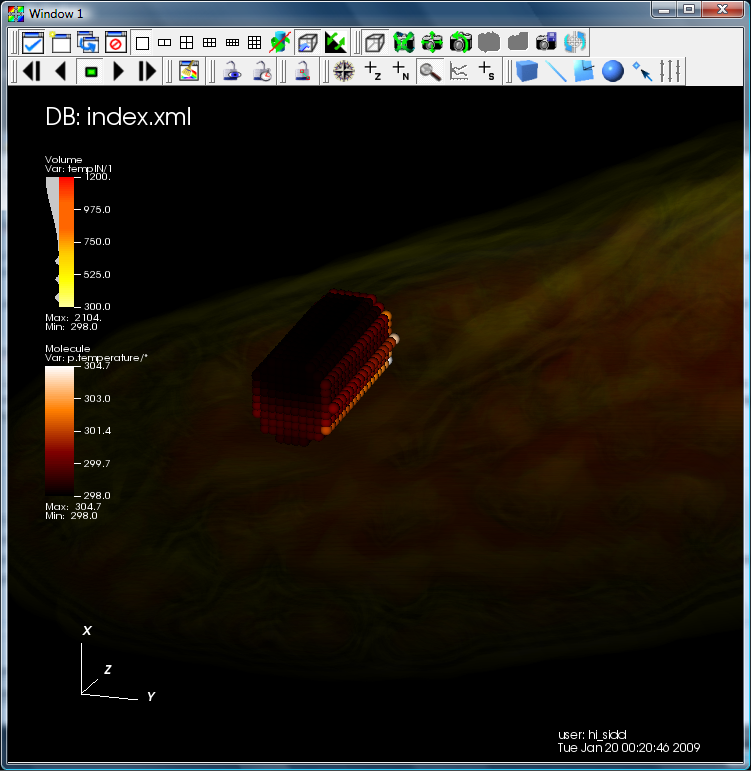
\includegraphics[width=.3\textwidth]{VisItMoleculePTtempViewer.png}}
 \vspace{-10pt}
  \caption{}
  \label{}
\end{figure}


% \begin{wrapfigure}{r}{.5\textwidth}
%   \center
%   \vspace{-30pt}
%   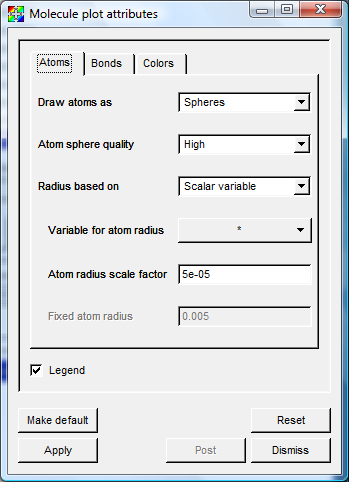
\includegraphics[width=.4\textwidth]{VisItMoleculeAttributesPTemp1.png}
%   \caption{Selecting a molecule plot and an associated variable/ material}
%   \label{VisItMoleculeAttributesPTemp1}
% \end{wrapfigure}

We choose to visualize the particles as Sphere Impostors (doesn't runs
the GPU out of memory, drawing as Spheres does). We also choose to
scale the sphere radius by a Scalar Variable and specify that variable
to be p.temperature/* itself (therefore the * appears). Since the
temperature values are too high, we scale them all by a factor of
5.e-05 (on the basis of trial and error). Finally in Colors tab, we
set the Color map for scalars as orangehot.  Combined with volume
visualization, we get a visualization as shown in
Figure~\ref{VisItMoleculePTtempViewer}.

% \begin{wrapfigure}{r}{100mm}
%   \center
%   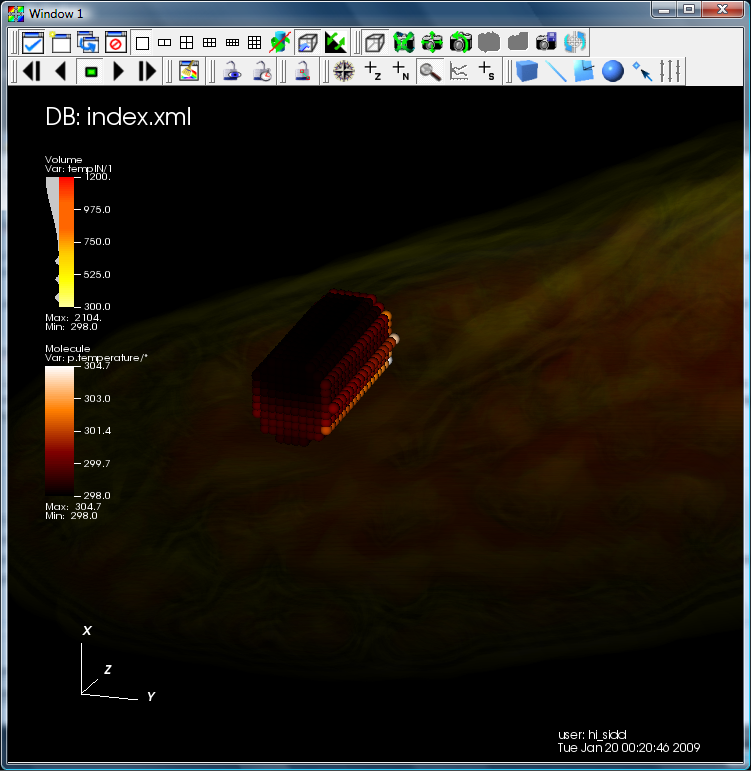
\includegraphics[width=.5\linewidth]{VisItMoleculePTtempViewer.png}
%   \caption{Selecting a molecule plot and an associated variable/ material}
%   \label{VisItMoleculePTtempViewer}
% \end{wrapfigure}

\subsection{Visualizing patch boundaries}
% In order to generate an image, like the one shown in
% Figure~\ref{VisItSubsetPlot}, we use the Subset plot. As with other
% variables, we select the Subset plot and an associated variable. The
% variables have a prefix 'level/ patch'. There is a level/ patch
% variable associated with every kind of variable (Cell Centered, Node
% Centered, Face Centeerd) present in the dataset. In the
% figure~\ref{VisItSubsetPlotVariables}, we select one such variable.
In order to visualize patch boundaries, we use the Subset plot. As
with other variables, we select the Subset plot and an associated
variable. The variables have a prefix 'level/ patch'. There is a
level/ patch variable associated with every kind of variable (Cell
Centered, Node Centered, Face Centered) present in the dataset. In the
Figure~\ref{VisItSubsetPlotVariables}, we select one such variable.
Next, we hit Draw. This produces a visualization as shown in
Figure~\ref{VisItSubsetPlotViewer}.

%\begin{figure}
%  \center
%  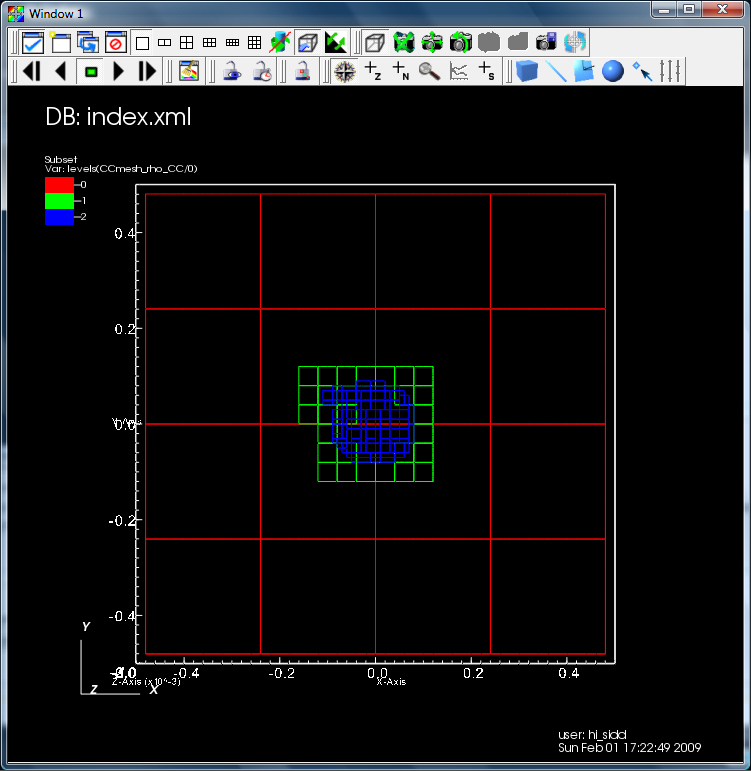
\includegraphics[scale=0.5]{VisItSubsetPlot.png}
%  \caption{Visualizing patch boundaries} 
%  \label{VisItSubsetPlot}
%\end{figure}

% \begin{wrapfigure}{r}{.5\textwidth}
%   \center
%   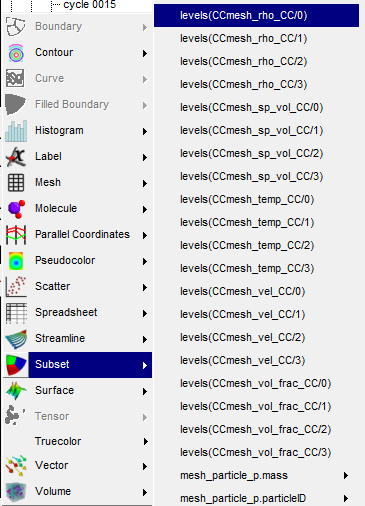
\includegraphics[width=.4\textwidth]{VisItSubsetPlotVariables.png}
%   \caption{A patch/ level variable, associated with every kind of variable}
%   \label{VisItSubsetPlotVariables}
% \end{wrapfigure}

\begin{figure}[h]
  \centering
 \subfloat[A patch/ level variable, associated with every kind of variable]{\label{VisItSubsetPlotVariables}
  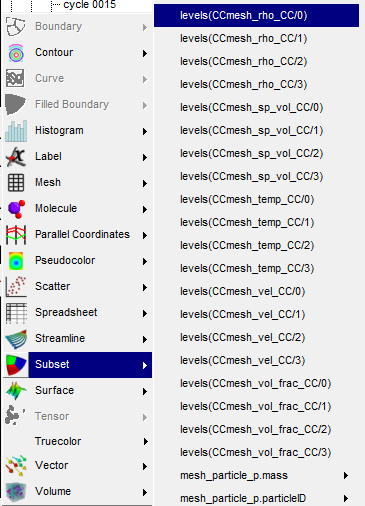
\includegraphics[width=.3\textwidth]{VisItSubsetPlotVariables.png}}
  \hspace{50pt}
 \subfloat[The default visualization of patches]{\label{VisItSubsetPlotViewer}
 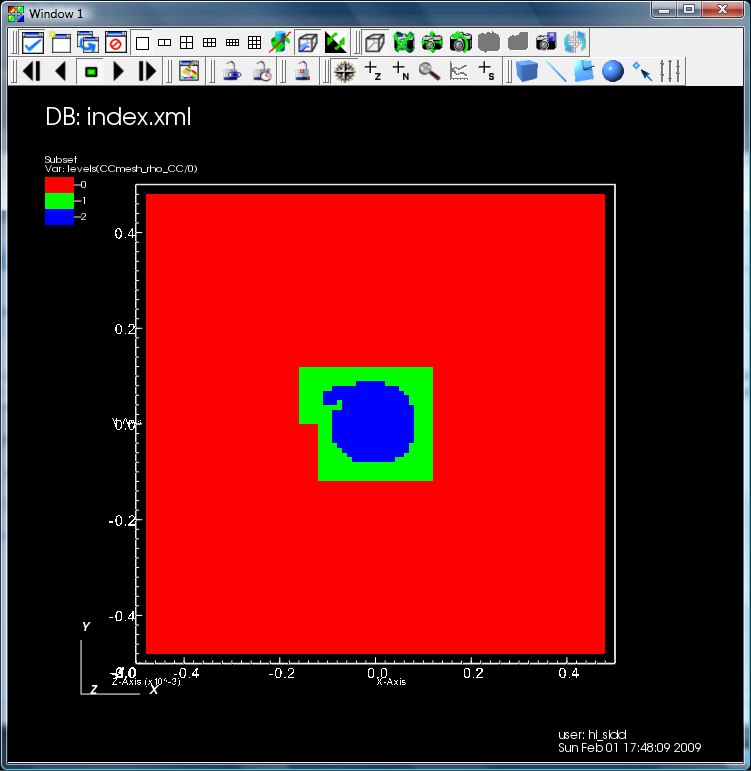
\includegraphics[width=.3\textwidth]{VisItSubsetPlotViewer.png}}
 \vspace{-20pt}
  \caption{}
  \label{}
\end{figure}



To generate a wire-frame model, we double click on the Subset plot in
the Active plots window. This pops up the Subset plot attributes
window, where we check the Wireframe mode as shown in
Figure`\ref{VisItSubsetPlotAttrib}. This would produce a
visualization, similar to one shown in
Figure~\ref{VisItSubsetPlotWireframe}.

% \begin{wrapfigure}{r}{.5\textwidth}
%   \center
%   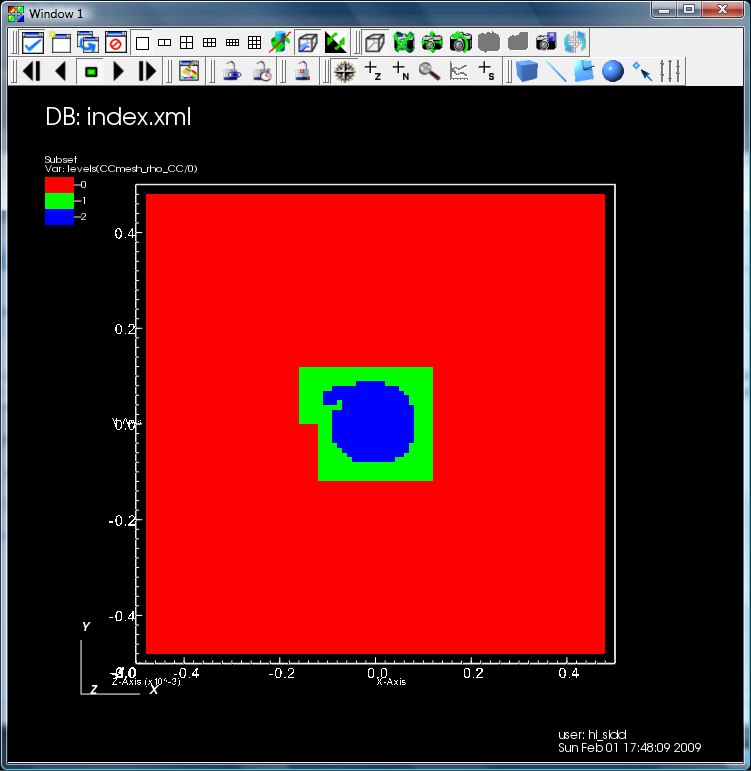
\includegraphics[width=.4\textwidth]{VisItSubsetPlotViewer.png}
%   \caption{The default visualization of patches} 
%   \label{VisItSubsetPlotViewer}
% \end{wrapfigure}

% \begin{wrapfigure}{r}{100mm}
%   \center
%   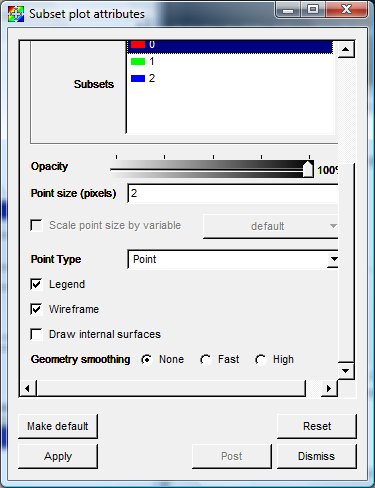
\includegraphics[width=.5\linewidth]{VisItSubsetPlotAttrib.png}
%   \caption{Enabling the 'Wireframe' mode for visualizing patch boundaries}
%   \label{VisItSubsetPlotAttrib}
% \end{wrapfigure}

% \begin{wrapfigure}{r}{100mm}
%   \center
%   \includegraphics[width=.5\linewidth]{VisItSubsetPlotWireframe.png}
%   \caption{The patch boundaries after enabling the wireframe mode}
%   \label{VisItSubsetPlotWireframe}
% \end{wrapfigure}

\begin{figure}[h]
  \centering
 \vspace{-5pt}
 \subfloat[Enabling the 'Wireframe' mode for visualizing patch boundaries]{\label{VisItSubsetPlotAttrib}
  \includegraphics[width=.25\textwidth]{VisItSubsetPlotAttrib.png}}
  \hspace{50pt}
 \subfloat[The patch boundaries after enabling the wireframe mode]{\label{VisItSubsetPlotWireframe}
 \includegraphics[width=.3\textwidth]{VisItSubsetPlotWireframe.png}}
 \vspace{-10pt}
  \caption{}
 \vspace{-10pt}
  \label{}
\end{figure}

\subsection{Iso-surfaces}

The easiest way to draw iso-surfaces is to use the 'Contour' Plot. As
with other plots demonstrated above, the contour plot is selected on a
regular 3D scalar variable. Figure ~\ref{VisItContourPlot} illustrates
this.

\begin{wrapfigure}{r}{.5\textwidth}
  \center
  \vspace{-35pt}
  \includegraphics[width=0.4\textwidth]{VisItContourPlot.png}
  \caption{Selecting the 'Contour' plot on a regular 3D scalar variable}
  \label{VisItContourPlot}
\end{wrapfigure}

Once the plot is selected, we hit 'Draw'. This would produce a
visualization, similar to one shown in
Figure~\ref{VisItContourPlotViewer}. You can then modify the plot
attributes by double clicking on the plot in the 'Active plots'
window. This would pop up the 'Contour plot attributes window', as
shown in Figure~\ref{VisItContourPlotAttrib}.

The 'Select by' option can be changed to 'Value(s)' and
'Percent(s)'. When specifying multiple values, they should be
separated by a space.


% \begin{wrapfigure}{r}{100mm}
%   \center
%   \includegraphics[scale=0.25]{VisItContourPlotViewer.png}
%   \caption{Iso-surface visualization}
%   \label{VisItContourPlotViewer}
% \end{wrapfigure}

% \begin{wrapfigure}{r}{100mm}
%   \center
%   \includegraphics[scale=0.5]{VisItContourPlotAttrib.png}
%   \caption{The attributes window for the 'Contour' plot}
%   \label{VisItContourPlotAttrib}
% \end{wrapfigure}

\begin{figure}[h]
  \centering
 \vspace{5pt}
 \subfloat[Iso-surface visualization]{\label{VisItContourPlotViewer}
  \includegraphics[width=.5\textwidth]{VisItContourPlotViewer.png}}
  \hspace{50pt}
 \subfloat[The attributes window for the 'Contour' plot]{\label{VisItContourPlotAttrib}
 \includegraphics[width=.25\textwidth]{VisItContourPlotAttrib.png}}
 \vspace{-10pt}
  \caption{}
 \vspace{-10pt}
  \label{}

\end{figure}


\subsection{Streamlines}

The 'Streamlines' plot has issues with the current version of VisIt
(1.11.2 and older). However, these have been corrected in the trunk
and should be out in version 2.0. The controls remain the same in all
these version and the example below was implemented on the trunk
version.

As shown in Figure~\ref{VisItStreamlinesPlot} we select the
'Streamlines' plot on a vector variable. We then double click on the
plot itself, which pops up the 'Streamlines attributes window'.

\begin{wrapfigure}{r}{.5\textwidth}
  \center
  \vspace{-10pt}
  \includegraphics[width=.4\textwidth]{VisItStreamlinesPlot.png}
  \caption{Selecting the 'Streamlines' plot on a vector variable}
  \label{VisItStreamlinesPlot}
\end{wrapfigure}

We set the 'Distance' parameter such that it covers the entire
computational domain. We set the 'Streamline direction' as forward. In
the 'Source' tab, Figure~\ref{VisItStreamlinesAttrib1}, we define the
'Source type' as 'Line'. We can select other options too, notably
'Single Point', 'Sphere' etc. We now define the line 'Start' and 'End'
coordinates. In this specific case, we define them as [-0.1 -0.05 0]
and [-0.1 0.05 0] respectively. This choice ensures that we cover the
entire y axis and start at the leftmost corner of the computational
domain.

To ensure that our stream lines are smooth, we change the 'Maximum
step length' in the in the 'Advanced' tab. In this case, we change it
to 1.e-05. The thing to keep in mind is that this length should be
order of magnitude smaller than the length of the computational
domain. This is shown in Figure ~\ref{VisItStreamlinesAttrib2}.

% \begin{wrapfigure}{r}{.5\textwidth}
%   \center
%   \includegraphics[width=.4\textwidth]{VisItStreamlinesAttrib1.png}
%   \caption{Setting the 'Source' tab parameters}
%   \label{VisItStreamlinesAttrib1}
% \end{wrapfigure}

% \begin{wrapfigure}{r}{.5\textwidth}
%   \center
%   \includegraphics[width=.4\textwidth]{VisItStreamlinesAttrib2.png}
%   \caption{Setting the 'Advanced' tab parameters}
%   \label{VisItStreamlinesAttrib2}
% \end{wrapfigure}

Once these parameters are set, we hit 'Apply' and then click on the 'Draw' button on the gui. This produces a visualization similar to one shown in Figure ~\ref{VisItStreamlinesViewer}.

% \begin{wrapfigure}{r}{100mm}
%   \center
%   \includegraphics[scale=0.4]{VisItStreamlinesViewer.png}
%   \caption{Streamlines visualization}
%   \label{VisItStreamlinesViewer}
% \end{wrapfigure}


\begin{figure}[h]
  \centering
 \vspace{5pt}
 \subfloat[Setting the 'Source' tab parameters]{\label{VisItStreamlinesAttrib1}
  \includegraphics[width=.25\textwidth]{VisItStreamlinesAttrib1.png}}
  \hspace{10pt}
 \subfloat[Setting the 'Advanced' tab parameters]{\label{VisItStreamlinesAttrib2}
 \includegraphics[width=.25\textwidth]{VisItStreamlinesAttrib2.png}}
 \hspace{10pt}
 \subfloat[Streamlines visualization]{\label{VisItStreamlinesViewer}
 \includegraphics[width=.4\textwidth]{VisItStreamlinesViewer.png}}
  \caption{}
 \vspace{-10pt}
  \label{}
\end{figure}


\subsection{Visualizing extra cells}

For visualizing extra cells we use the 'Inverse Ghost Zone' operator
~\ref{VisItInverseGhostZoneOp} in conjunction with the 'Pseudocolor'
plot. Since the plugin reads in extra cells as ghost cells, the usage
of this operator make sense in this scenario.

% \begin{wrapfigure}{r}{.5\textwidth}
%   \center
%   \vspace{-20pt}
%   \includegraphics[width=0.15\textwidth]{VisItInverseGhostZoneOp.png}
%   \caption{Selecting the Inverse Ghost Zone operator}
%   \label{VisItInverseGhostZoneOp}
% \end{wrapfigure}

After the operator is applied to the 'Pseudocolor' plot, we double
click on the operator to change its attributes. We switch to 'Both
ghost zones and real zones' in this window
~\ref{VisItInverseGhostZoneAttribs} and hit 'Apply'.

% \begin{wrapfigure}{r}{.5\textwidth}
%   \center
%   \includegraphics[width=0.4\textwidth]{VisItInverseGhostZoneAttribs.png}
%   \caption{The attributes window for the 'Inverse Ghost Zone' operator}
%   \label{VisItInverseGhostZoneAttribs}
% \end{wrapfigure}

We then hit 'Draw'. When combined with the 'Mesh' plot we get a visualization similar to the one shown in Figure ~\ref{VisItInverseGhostZoneViewer}. The pick operations on the viewer can then be used to investigate the value(s) in these extra cells. 

% \begin{wrapfigure}{r}{.5\textwidth}
%   \center
%   \includegraphics[width=0.4\textwidth]{VisItInverseGhostZoneViewer.png}
%   \caption{Extra cells together with the 'Mesh' plot}
%   \label{VisItInverseGhostZoneViewer}
% \end{wrapfigure}

\begin{figure}[h]
  \centering
 \vspace{5pt}
 \subfloat[Selecting the Inverse Ghost Zone operator]{\label{VisItInverseGhostZoneOp}
  \includegraphics[width=.15\textwidth]{VisItInverseGhostZoneOp.png}}
  \hspace{20pt}
 \subfloat[The attributes window for the 'Inverse Ghost Zone' operator]{\label{VisItInverseGhostZoneAttribs}
 \includegraphics[width=.25\textwidth]{VisItInverseGhostZoneAttribs.png}}
 \hspace{20pt}
 \subfloat[Extra cells together with the 'Mesh' plot]{\label{VisItInverseGhostZoneViewer}
 \includegraphics[width=.45\textwidth]{VisItInverseGhostZoneViewer.png}}
  \caption{}
 \vspace{-10pt}
  \label{}
\end{figure}


\subsection{Picking on particles}

The 'Node pick mode' on the visualization window can be used to pick
particles and investigate particles attributes. After plotting
particles using the 'Molecule' plot, the user can then select the
'Node pick mode' ~\ref{VisItNodePick} and select particles (by
clicking on them) of interest.

 \begin{wrapfigure}{r}{.5\textwidth}
   \center
   \includegraphics[width=0.5\textwidth]{VisItNodePick.png}
   \caption{The 'Node pick mode' on the visualization window}
   \label{VisItNodePick}
 \end{wrapfigure}

Once a particle is picked, the 'Pick' window pops up with the particle
attributes. By default only the variable plotted is queried, if the
user wants to query more variables per pick - they can be added by
selecting additional variables from the 'Variables' menu and as shown
in the Figure ~\ref{VisItPickWindow}.

% \begin{wrapfigure}{r}{.5\textwidth}
%   \center
%   \includegraphics[width=0.4\textwidth]{VisItPickWindow.png}
%   \caption{The 'Pick' window }
%   \label{VisItPickWindow}
% \end{wrapfigure}

% \begin{figure}[h]
%   \centering
%  \vspace{5pt}
%  \subfloat[The 'Node pick mode' on the visualization window]{\label{VisItNodePick}
%   \includegraphics[width=.4\textwidth]{VisItNodePick.png}}
%   \hspace{20pt}
%  \subfloat[The 'Pick' window]{\label{VisItPickWindow}
%  \includegraphics[width=.4\textwidth]{VisItPickWindow.png}}
%   \caption{}
%  \vspace{-10pt}
%   \label{}
% \end{figure}

\begin{figure}[h]
  \centering
  \includegraphics[width=.4\textwidth]{VisItPickWindow.png}
  \caption{The 'Pick' window}
  \label{VisItPickWindow}
\end{figure}

\subsection{Selectively visualizing vectors}
The expression editor can be used to define a vector variable with magnitude greater or lesser than a certain extent. An example of this is shown below,

\begin{verbatim}
if(gt(magnitude(<vel_CC/1>), 0.0), <vel_CC/1>, {0, 0, 0})
\end{verbatim}

Put into words, if magnitude of vel\_CC/1 is greater than 0.0, display it, else display a zero magnitude vector. To use the 'lesser than' parameter, replace 'gt' with 'lt'.

%\chapter{Visualization Tools -- Manta}

%To run the C-SAFE scene: 
%\begin{Verbatim}[fontsize=\footnotesize]
%  Manta/build/bin/csafe_scene
%\end{Verbatim}

%The csafescene window will open showing a transfer function editor.  To add files to load run:
%\begin{Verbatim}[fontsize=\footnotesize]
%  File -> Add/Remove NRRD Files
%\end{Verbatim}

%\begin{figure}[htbp]
%  \center
%  \includegraphics[width=.5\linewidth]{manta_files.png}
%  \caption{Opening the scene}
%  \label{fig:manta_files}
%\end{figure}

% This will open a window where you can add volume and particle files in .nrrd or .nhdr formats.  Select add particle file(s) and open a particle nrrd file in .nhdr or .nrrd format.  These nrrd files should be created with the uda2nrrd tool.

% \begin{figure}[htbp]
%   \center
%   \includegraphics[width=.5\linewidth]{manta_add_files.png}
%   \caption{Adding files to the scene}
%   \label{fig:manta_add_files}
% \end{figure}

% A similarly named volume nrrd should be automatically added if in the same folder.  Close the window by pressing "OK".  The files won't be loaded yet so you can make modifications to the data to be loaded in before loading them.  To load the files:

% \begin{Verbatim}[fontsize=\footnotesize]
%   Scene -> Generate
% \end{Verbatim}

% The resulting csafe scene window should look similar to:

% \begin{figure}[htbp]
%   \center
%   \includegraphics[width=.5\linewidth]{manta_histograms.png}
%   \caption{C-SAFE window with histograms from loaded nrrd files}
%   \label{fig:manta_histograms}
% \end{figure}

% and a separate window will open showing the visualization. 

% \section{Manta Commandline options} 
% Many of the operations typically used through the GUI can be used through the commandline when running the csafe scene.

% \begin{enumerate}

% \item
% --np=<int>  : the number of processes to devote to Manta. Should be roughly equivalent to the number of cores in your system.
% \item
% --cfg=<string>  : load a configuration file, this has histogram and filenames saved
% \item
% --nrrdlist=<string>  : load a nrrdlist
% \item
% --uda=<string>  : load an UDA file
% \item
% --res <int>x<int>: resolution of window, ie 512x512
% \item
% --g  : generate (load) all datasets when starting up, should be used in conjunction with --nrrdlist or --cfg

% \end{enumerate}

% Additionally, many of the commandline options that Manta uses can also be used with the csafe scene.  These commands configure rendering options.  For example, jittered sampling may reduce aliasing effects.

% \begin{enumerate}

% \item
% --imagetype <string> : manta image type (see manta command line options)
% \item
% --shadows <string> : manta shadow algorithm (see manta command line options)
% \item
% --imagetraverser <string> : manta image traverser (see manta command line options)
% \item
% --loadbalancer <string> : manta load balancer option (see manta command line options)
% \item
% --renderer <string> : manta renderer (see manta command line options)


% \end{enumerate}

% \section{Saving and Loading}

% You can save the status of your project through File->Save or File->save as. Note that saving your project saves everything from the clipping regions to the transfer functions but currently does not save some things such as the background color or the camera position.

% Exporting transfer functions: You can export the transfer function currently displayed by selecting File->Export Transfer Function. This is The exported format is as follows: position r g b a position r g b a ... position is a number (0-1) that specifies the position of your control point in the transfer function. r g b a are simply the color and alpha values of the control point.

% You can import saved transfer functions from File->import Transfer Function. 

% The configuration file saves the data files used however if you would like to use the same configuration file for multiple sets of data you can select File->Export NrrdList.  This stores the data files as a list in ASCII which can be imported to use with any configuration.  

% \section{Using the Transfer Function Editor}

% \begin{figure}[htbp]
%   \center
%   \includegraphics[width=.5\linewidth]{transferF.png}
%   \caption{Transfer function editor.}
%   \label{fig:manta_tf}
% \end{figure}

% The transfer function display in the histogram window displays the currently selected transfer function. To select a different transfer function, click on the color wheel icon next to the histogram. The transfer function can be modified in a similar fashion to gradient editors in popular image editing programs. The color and opacity of the data range can be adjusted by modifying the control points. The default transfer function is a rainbow. To change a color, select a control point and click the color wheel to edit it. Or you can simply right-click on a control point to change the color. To modify opacity, simply move the control points up and down by clicking and dragging them.

% \section{Histogram Controls}

% \begin{figure}[htbp]
%   \center
%   \includegraphics[width=.5\linewidth]{histogram.png}
%   \caption{Histogram with controls.}
%   \label{fig:manta_histogram}
% \end{figure}

% Histograms represent the frequency of data values in a data set. Each histogram is associated with an index into either a volume or sphere data. If you select index 0 in the sphere data set, then the histogram mostly likely shows the accumulated range of x-coordinates for all of the sphere data sets. There is a semi-transparent grey box overlaying each histogram. This represents the range of values in the histogram that are displayed. Clicking on the right or left side of this box moves the left or right side of the clipping region accordingly. You can also click and drag the middle of the region to drag the region along the histogram. You can also use the mouse wheel to zoom into a region of the histogram.
%   Name (\#) - The name associated with the histogram and the index it corresponds to in the NRRD file. 
% To the right are various controls.

% \begin{enumerate}
% \item
% colorwheel : This will make this histogram's transfer function display in the transfer function panel and also make it the active transfer function for either the volume or sphere data.
% \item
% Ruler : you can explicitly set specific data ranges for the clipping region or the region of the data to which the transfer function applies to. This is extremely useful if there is only a vary narrow region of the data range that you want to be looking at.
% \item
% Zoom in/out: this will zoom in to the clipping region or back out to the zoom where you were previously. 
% \end{enumerate}

% \section{Ambient Occlusion}
%   Ambient occlusion is an approximation of global illumination and can give a better sense of relative depth in clusters of objects.  To enable ambient occlusion turn it on in Scene->Preferences.  There are two variables to modify, the cutoff distance and the number of rays shot.  The cutoff distance is how far away objects can be to occlude rays.  To produce a good image it is a good idea to turn off the volume and reduce or remove the lights.  The light can be turned off in the Light dialog in the Manta Menu.  Setting the light color to black will completely disable a light.
  
% %\section{CSAFE Window Menus}

% % \subsection{File - Save and Load Configuration File}

% % \subsection{File - Save and Load NRRDFile}

% % \subsection{File - Add Remove NRRD Files}

% % \subsection{File - Import Export Transfer Function}

% % \subsection{Scene - Add Histogram}

% % \subsection{Scene - Scene Preferences}

% % \subsection{Scene - Volume Position Size}

% % \subsection{Scene - Cutting Bounding Box}

% % \subsection{Scene - Generate}

% % \section{Manta Window Menus}

% % \subsection{File - Threads}

% % \subsection{Camera - Auto View}

% % \subsection{Camera - Edit Camera}

% % \subsection{Camera - Edit Background}

% % \subsection{Camera - Camera Paths}

% % \subsection{Camera - Capture Frames}

% % \subsection{Lights - Edit Lights}

% % \subsection{Lights - Enable Visible Lights}


% \section{Manta FAQ}

% \begin{enumerate}
% \item
% Q. "I get an error Gtk-CRITICAL **: file gtkrange.c".
% A.  This error pops up on some system and can safely be ignored.
% Q.  "It is running very slowly"
% A.  Try increasing the number of threads, shrinking the window size, and reducing the step size through the volume.
% \end{enumerate}


%__________________________________
\chapter{Data Extraction Tools}

Uintah offers a number of tools for accessing data stored in Uintah
Data Archives (``UDAs").  Because the format of Uintah data is
specific to the framework, these tools allow a user to quickly extract
data, which can then either be postprocessed within that tool (simple
modification of the source code may be necessary), postprocessed with
external software such as Matlab or Octave, or simply plotted with,
e.g. gnuplot.  These tools are not compiled automatically when ``make
sus'' is issued.  To compile them cd to ``opt/StandAlone/tools'' and
issue ``make''.  These tools are described below.

\section{puda}

The command line extraction utility \tt puda \normalfont (for ``parse
Uintah data archive") has a number of uses.  For example, it may be
used to extract a subset of particle data from a UDA.  Once the
extraction tools have been compiled, the puda executable will be
located in \tt opt/StandAlone/tools/puda/. \normalfont If the
executable is run with no additional command line arguments, the
following usage information will be displayed:

\begin{Verbatim}[fontsize=\footnotesize]
Usage: puda [options] <archive file>

Valid options are:
  -h[elp]
  -timesteps
  -gridstats
  -listvariables
  -varsummary
  -jim1
  -jim2
  -partvar <variable name>
  -asci
  -tecplot <variable name>
  -no_extra_cells     (Excludes extra cells when iterating over cells.
                       Default is to include extra cells.)
  -cell_stresses
  -rtdata <output directory>
  -PTvar
  -ptonly             (prints out only the point location
  -patch              (outputs patch id with data)
  -material           (outputs material number with data)
  -NCvar <double | float | point | vector>
  -CCvar <double | float | point | vector>
  -verbose            (prints status of output)
  -timesteplow <int>  (only outputs timestep from int)
  -timestephigh <int> (only outputs timesteps up to int)
  -matl,mat <int>         (only outputs data for matl)
*NOTE* to use -PTvar or -NVvar -rtdata must be used
*NOTE* ptonly, patch, material, timesteplow, timestephigh are used in conjunction with -PTvar.
\end{Verbatim}

As an example of how to use \tt puda, \normalfont suppose that one
wanted to know the locations of all particles at the last archived
timestep for the \tt const\_test\_hypo.uda \normalfont First one may
wish to know how many timesteps have been archived.  This could be
accomplished by:

\begin{Verbatim}[fontsize=\footnotesize]
 puda -timesteps const_test_hypo.uda
\end{Verbatim}
The resulting terminal output would be:
\begin{Verbatim}[fontsize=\footnotesize]
Parsing const_test_hypo.uda/index.xml
There are 11 timesteps:
1: 1.8257001926347728e-05
548: 1.0012914931998474e-02
1094: 2.0005930425875382e-02
1640: 3.0015616802173569e-02
2184: 4.0005272397960444e-02
2728: 5.0011587657447343e-02
3271: 6.0016178181543284e-02
3812: 7.0000536667661845e-02
4353: 8.0001537138146825e-02
4893: 9.0000702723306208e-02
5433: 1.0001655973087024e-01
\end{Verbatim}

These represent all of the timesteps for which data has been archived.
Suppose now that we wish to know what the stress state is for all
particles (in this case two) at the final archived timestep.  For this
one could issue:

\begin{Verbatim}[fontsize=\footnotesize]
puda -partvar p.stress -timesteplow 10 -timestephigh 10 const_test_hypo.uda
\end{Verbatim}

The resulting output is:

\begin{Verbatim}[fontsize=\footnotesize]
Parsing const_test_hypo.uda/index.xml
1.00016560e-01 1 0 281474976710656 -2.72031498e-10 -1.05064208e-26 -2.53781271e-08 -1.05064208e-26 -2.72031498e-10 -1.23584688e-09 -2.53781271e-08 -1.23584688e-09 1.63840079e-07
1.00016560e-01 1 1 0 1.93256890e-13 6.56787331e-18 1.85514400e-14 6.56787331e-18 2.24310469e-13 1.85519650e-14 1.85514400e-14 1.85519650e-14 -3.20052991e+06
\end{Verbatim}

The first column is the simulation time, the third column is the
material number, the fourth column is the particle ID, and the
remaining nine columns represent the components of the Cauchy stress
tensor ($ \sigma_{11}$,$\sigma_{12}$,$\sigma_{13}$, ...,
$\sigma_{32}$,$\sigma_{33}$).  If desired, the terminal output can be
redirected to a text file for further use.

\section{partextract}

The command-line utility \tt partextract \normalfont may be used to
extract data from an individual particle.  To do this you first need
to know the ID number of the particle you are interested in.  This may
be done by using the puda utility, or the visualization tools.  Once
the extraction tools have been compiled, the partextract utility
executable will be located in \tt /opt/StandAlone/tools/extractors/
\normalfont.  If the executable is run without any arguments the
following usage guide will be displayed in the terminal:

\begin{Verbatim}[fontsize=\footnotesize]
No archive file specified
Usage: partextract [options] <archive file>

Valid options are:
  -mat <material id>
  -partvar <variable name>
  -partid <particleid>
  -part_stress [avg or equiv or all]
  -part_strain [avg/true/equiv/all/lagrangian/eulerian]
  -timesteplow [int] (only outputs timestep from int)
  -timestephigh [int] (only outputs timesteps upto int)
\end{Verbatim}

As an example of how to use the partextract utility, suppose we wanted
to find the velocity at every archived timestep for the particle with
ID 281474976710656 (found above using puda) in the
``const\_test\_hypo.uda'' file (src/StandAlone/inputs/MPM).  The
appropriate command to issue is:

\begin{Verbatim}[fontsize=\footnotesize]
partextract -partvar p.velocity -partid 281474976710656 const\_test\_hypo.uda
\end{Verbatim}

The output to the terminal is:

\begin{Verbatim}[fontsize=\footnotesize]
Parsing const_test_hypo.uda/index.xml
1.82570019e-05 1 0 281474976710656 0.00000000e+00 0.00000000e+00 -1.00000000e-02
1.00129149e-02 1 0 281474976710656 -1.03554318e-19 -1.03554318e-19 -1.00000000e-02
2.00059304e-02 1 0 281474976710656 -1.99388121e-19 -1.99388121e-19 -1.00000000e-02
	.
	.
	.
\end{Verbatim}

It is noted that if the stress tensor is output using the partextract utility, the output format is different than for the puda utility.  The partextract utility only outputs the six independent components instead of all nine.  For example, if we use partextract to get the stress tensor for the same particle as above at the last archived timestep only, the output is:

\begin{Verbatim}[fontsize=\footnotesize]
partextract -partvar p.stress -partid 281474976710656 -timesteplow 10 -timestephigh 10 const_test_hypo.uda
Parsing const_test_hypo.uda/index.xml
1.00016560e-01 1 0 281474976710656 -2.72031498e-10 -1.05064208e-26 -2.53781271e-08 -1.05064208e-26 -2.72031498e-10 -1.23584688e-09 -2.53781271e-08 -1.23584688e-09 1.63840079e-07
\end{Verbatim}

Compare this output with the output from puda above.  Notice that the
ordering of the six independent components of the stress tensor for
partextract are $\sigma_{11}$,$\sigma_{22}$, $\sigma_{33}$,
$\sigma_{23}$, $\sigma_{13}$ , $\sigma_{12}$.

\section{lineextract}

Lineextract is used to extract an array of data from a region of a
computational domain. Data can be extracted from a point, along a
line, or from a three dimensional region and then stored as a variable
for ease of post processing.

Usage: \begin{Verbatim}[fontsize=\footnotesize]
./lineextract [options] -uda <archive file>

Valid options are:
 -h,        --help
 -v,        --variable:      <variable name>
 -m,        --material:      <material number> [defaults to 0]
 -tlow,     --timesteplow:   [int] (sets start output timestep to int) [defaults to 0]
 -thigh,    --timestephigh:  [int] (sets end output timestep to int) [defaults to last timestep]
 -timestep, --timestep:      [int] (only outputs from timestep int) [defaults to 0]
 -istart,   --indexs:        <x> <y> <z> (cell index) [defaults to 0,0,0]
 -iend,     --indexe:        <x> <y> <z> (cell index) [defaults to 0,0,0]
 -l,        --level:         [int] (level index to query range from) [defaults to 0]
 -o,        --out:           <outputfilename> [defaults to stdout]
 -vv,       --verbose:       (prints status of output)
 -q,        --quiet:         (only print data values)
 -cellCoords:                (prints the cell centered coordinates on that level)
 --cellIndexFile:             <filename> (file that contains a list of cell indices)
                                  [int 100, 43, 0]
                                  [int 101, 43, 0]
                                  [int 102, 44, 0]
\end{Verbatim}

The following example shows the usage of lineextract for extracting
density data at the 60th computational cell in the x-direction,
spanning the width of the domain in the y-direction (0 to 1000), at
timestep, 7, (note ``timestep" actually refers to the seventh data
dump, not necessarily the seventh timestep in the simulation. The
variable containing the density data within the uda is ``rho\_CC," and
the output variable that will store the data for post processing is
``rho."
\begin{Verbatim}[fontsize=\footnotesize]
./lineextract -v rho_CC  -timestep 7 -istart 60 0 0 -iend 60 1000 0 -m 1 -o rho -uda test01.uda.000
\end{Verbatim}

%__________________________________
\section{compute\_Lnorm\_udas}
\TT{Compute\_Lnorm\_udas} computes the $L_1$, $L_2$ and $L_\infty$
norms for each variable in two udas.  This utility is useful in
monitoring how the solution differs from small changes in either the
solution tolerances, input parameters or algorithmic changes.  You can
also use it to test the domain size influence.  The norms are computed
using:
%
\begin{equation}
  d[i] = |uda_1[i] - uda_2[i]|
\end{equation}
%
\begin{equation}
  L_1 = \frac{\raise1.5pt\hbox{$\sum_i^\text{All Cells}$}d[i]}{\text{number of cells}}
\end{equation}
%
\begin{equation}
  L_2 = \sqrt{ \frac{\raise1.5pt\hbox{$\sum_i^\text{All Cells}$}d[i]^2}{\text{number of cells}} }
\end{equation}
%
\begin{equation}
  L_\infty = \text{max}(d[i])
\end{equation}
%
These norms are computed for each \TT{CC, NC, SFCX, SFCY, SFCZ}
variable, on each level for each timestep.  The output is displayed on
the screen and is placed in a directory named `Lnorm.'  The directory
structure is:
%
\begin{Verbatim}[fontsize=\footnotesize]
 Lnorm/
   -- L-0
    |-- delP_Dilatate_0
    |-- mom_L_ME_CC_0
    |-- press_CC_0
    |-- press_equil_CC_0
    |-- variable
    |-- variable
    |--etc
\end{Verbatim}
%
and in each variable file is the physical time, $L_1$, $L_2$ and $L_\infty.$  These data can be plotted using \TT{gnuplot} or another plotting program.

The command usage is
%
\begin{Verbatim}[fontsize=\footnotesize]
  compute_Lnorm_udas <uda1> <uda2>
\end{Verbatim}
%
The utility allows for \TT{udas} that have different computational
domains and different patch distributions to be compared.  The uda
with the smallest computational domain should always be specified
first.
%
In order for the norms to be computed the physical times must satisfy 
\begin{equation*}
| \text{physical Time}_{uda_1} - \text{physical Time}_{uda_2}| < 1e^{-5}.
\end{equation*} 

%__________________________________
\section{timeextract} 

Timeextract is used to extract a user specified variable from a point in a computational
domain.  

Usage: \begin{Verbatim}[fontsize=\footnotesize]
./timeextract [options] -uda <archive file>

Valid options are:
  -h,--help
  -v,--variable <variable name>
  -m,--material <material number> [defaults to 0]
  -tlow,--timesteplow [int] (only outputs timestep from int) [defaults to 0]
  -thigh,--timestephigh [int] (only outputs timesteps up to int) [defaults to last timestep]
  -i,--index <x> <y> <z> (cell coordinates) [defaults to 0,0,0]
  -p,--point <x> <y> <z> [doubles] (physical coordinates)
  -l,--level [int] (level index to query range from) [defaults to 0]
  -o,--out <outputfilename> [defaults to stdout]
  -vv,--verbose (prints status of output)
  -q,--quite (only print data values)
  -noxml,--xml-cache-off (turn off XML caching in DataArchive)
 \end{Verbatim} 

The following example shows the usage of timeextract for extracting density data
at the computationat cell coordinates 5,0,0, from timestep 0 to the last
timestep. The variable containing the density data within the uda is "rho\_CC" and the output variable that
will store the data for post processing is "rho." 
\begin{Verbatim}[fontsize=\footnotesize]
./timeextract -v rho_CC -i 5 0 0 -o rho -uda test01.uda.000
\end{Verbatim}

%__________________________________
\section{particle2tiff} 
particle2tiff is used to extract a user specified particle variable,
compute a cell centered average and write that data to a series of tiff
slices that can be used in further image processing.  Each slice in the tiff
file corresponds to a plane in $z$ direction in the computational domain.
Each pixel in the tiff image represents a cell in the computational domain.
This utility depends on \TT{libtiff4, libtiff4-dev, \& libtiffxx0c2}, please
verify that they are installed on your system before configuring and compiling.


  
The data types supported are\TT{ double, Vector, Matrix3}, and the equations for computing the cell-centered average are:
\begin{eqnarray}
  CC_{ave} =& {\raise1.5pt\hbox{$\scriptstyle\sum_{p=1}^{nParticles}$}} Double[p]          \over {nParticles} \nonumber \\
  CC_{ave} =& {\raise1.5pt\hbox{$\scriptstyle\sum_{p=1}^{nParticles}$}} Vector[p].length() \over {nParticles} \nonumber \\
  CC_{ave} =& {\raise1.5pt\hbox{$\scriptstyle\sum_{p=1}^{nParticles}$}} Matrix3[p].Norm()  \over {nParticles}\nonumber
\end{eqnarray}

\noindent The usage is
\begin{Verbatim}[fontsize=\footnotesize]
Usage: tools/extractors/particle2tiff [options] -uda <archive file>

Valid options are:
  -h,        --help
  -v,        --variable:      [string] variable name
  -m,        --material:      [int or string 'a, all'] material index [defaults to 0]

  -max                        [double] (maximum clamp value)
  -min                        [double] (minimum clamp value)
  -orientation                [string] (The orientation of the image with respect to the rows and columns.)
                                      Options:
                                        topleft  0th row represents the ........
                                        topright 0th row represents the ........
                                        botright 0th row represents the ........
                             default->  botleft  0th row represents the .........
                                        lefttop  0th row represents the ........
                                        righttop 0th row represents the ........
                                        rightbot 0th row represents the ........
                                        leftbot  0th row represents the ........
                                                    Many readers ignore this tag
                                                    
  -tlow,     --timesteplow:   [int] (start output timestep) [defaults to 0]
  -thigh,    --timestephigh:  [int] (end output timestep) [defaults to last timestep]
  -timestep, --timestep:      [int] (only outputs timestep)  [defaults to 0]

  -istart,   --indexs:        <i> <j> <k> [ints] (starting point, cell index) [defaults to 0 0 0]
  -iend,     --indexe:        <i> <j> <k> [ints] (end-point, cell index) [defaults to 0 0 0]
  -startPt                    <x> <y> <z> [doubles] (starting point in physical coordinates)
  -endPt                      <x> <y> <z> [doubles] (end-point in physical coordinates)

  -l,        --level:         [int] (level index to query range from) [defaults to 0]
  -d,        --dir:           output directory name [none]
  --cellIndexFile:            <filename> (file that contains a list of cell indices)
                                   [int 100, 43, 0]
                                   [int 101, 43, 0]
                                   [int 102, 44, 0]
----------------------------------------------------------------------------------------
 For particle variables the average over all particles in a cell is returned.
 \end{Verbatim} 

The following example shows the usage of particle2tiff for averaging the particle stress (p.stress)
for all materials over the interior cells of the computational domain.  A series of 3 tiff slices 
are saved for every timestep in the directory``output." 
\begin{Verbatim}[fontsize=\scriptsize]
tools/extractors/particle2tiff -m all -d output -v p.stress -uda disks2mat4patch.uda.000/
There are 14 timesteps
 Initializing time_step_upper to 13
Removed directory: output
Created directory: output
Timestep[0] = 2.08084e-05
  p.stress: ParticleVariable<Matrix3> being extracted and averaged for material(s): 0, 1,  ........
  writing slice: [0/3] width: 256 height 256
  writing slice: [1/3] width: 256 height 256
  writing slice: [2/3] width: 256 height 256
Timestep[1] = 0.0100184
  p.stress: ParticleVariable<Matrix3> being extracted and averaged for material(s): 0, 1,  ........
  writing slice: [0/3] width: 256 height 256
  writing slice: [1/3] width: 256 height 256
  writing slice: [2/3] width: 256 height 256
Timestep[2] = 0.0200161
  p.stress: ParticleVariable<Matrix3> being extracted and averaged for material(s): 0, 1,  ........
  writing slice: [0/3] width: 256 height 256
  writing slice: [1/3] width: 256 height 256
  writing slice: [2/3] width: 256 height 256
Timestep[3] = 0.0300137
  p.stress: ParticleVariable<Matrix3> being extracted and averaged for material(s): 0, 1,  ........
  writing slice: [0/3] width: 256 height 256
  writing slice: [1/3] width: 256 height 256
  writing slice: [2/3] width: 256 height 256
\end{Verbatim}
A montage showing the average particle stress computed from particle2tiff is shown
in Fig. \ref{fig:p2tiff}.  In this simulation two similar disks collided at the center of the domain.
\vspace{-0.5in}
\begin{figure}
  \includegraphics[scale=.60]{particle2tiff.png}
  \caption{Montage showing the averaged particle stress for two cylindrical disks colliding.}
  \label{fig:p2tiff}
\end{figure}


%__________________________________
\section{On the fly analysis} 
On the fly analysis is used to determine the minimum and maximum of specified variables while the simulation is running.  Parameters are included in the input file to specify at what frequency the data is analyzed and which variables to look at. A new directory will be made in the uda directory for each level (e.g. L-0). Within the new directory the max and min of each variable for the specified material is determined as a function of time at the given sampling frequency. 

\begin{center}
\begin{tabular}{| l | c | p{7cm} |}
\hline
  \multicolumn{3}{|c|}{\textbf{Dynamic Output Intervals Input Parameters}} \\
\hline
\hline
  \textbf{Tag} & \textbf{Type} & \textbf{Description}\\
\hline
  $<$samplingFrequency$>$ & double & Sampling frequency in times per simulated second\\
\hline
  $<$timeStart$>$ & double & Simulation time when sampling begins (sec)\\
\hline
  $<$timeEnd$>$ & double & Simulation time when sampling ends (sec)\\
\hline
  $<$Variables$>$ & String & Variables to be analyzed including a specification for which material\\
\hline
\end{tabular}
\end{center}


The input file specification is as follows:
\begin{verbatim}
<DataAnalysis>
  <Module name = "minMax">
    <samplingFrequency> 1e8 </samplingFrequency>
    <timeStart> 0 </timeStart>
    <timeEnd> 1000 </timeEnd>
    <Variables>
      <analyze label="press_CC" matl="0"/>
      <analyze label="vel_CC" matl="1"/>
      <analyze label="rho_CC" matl="0"/>
    </Variables>
  </Module>
</DataAnalysis>
\end{verbatim}

\chapter{Order of Accuracy}
\label{chap:OA}

Order of accuracy is an extremely powerful framework that has been built to run a series of tests where multiple parameters are varied. The framework was originally built to easily do an order of accuracy analysis when resoultion was varied for a specific simulation. Since then it has been used for a variety of other tasks. The framework allows multiple tests to be easily repeated autonomously, proving to be extremely usefull for man studies. 

\section{Using The Framework}

The first step in using the framework, is to set up the tests you wish to run. All the assets this framework uses are located inside $\TT{/src/orderAccuracy/}$. $\TT{framwork\_scripts}$ contains all the scripts the framework uses to run, $\TT{postProcessTools}$ contains all the post processing scripts the study will use, and $\TT{test\_config\_files}$ contains all the studies which the framework can run. The framework has the ability to run any of .tst files located here. \\

To run a study using the order of accuracy tools, edit the $\TT{components.xml}$ inside of $\TT{test\_config\_files}$. All of the components (ICE MPM MPMICE Arches Wasatch) should be commented out, un-comment any component you wish to use. Next go into the directory for whichever component you un-commented. In this directory are all the available tests for that component and symbolic links to all the associated input files. To run these studies, edit $\TT{whatToRun.xml}$ and un-comment any simulations you would like to run.

Once all of the above steps have been done, you can follow these steps to run your studies.
\begin{enumerate}

\item cd to /opt/StandAlone or /dbg/StandAlone 
\item Create a symbolic link to orderAccuracy \\
\TT{ln -s /src/orderAccuracy}
\item Set a readlink to the orderAccuracy directory using the following command \\
\TT{set OA = `readlink -f orderAccuracy/`}
\item Run the following command to run your study
\begin{verbatim}
orderAccuracy/framework_scripts/masterScript.pl $OA
\end{verbatim}

\end{enumerate}

This will create a directory called $\TT{order\_of\_accuracy}$ which will contain all the studies you have run. WARNING - if you re-run any studies the framework with write over this directory, completely destroying anything that was previously there, so it is suggested to quickly move any data out of this directory.

\section{Tests}

The order of accuracy framework uses test or .tst files to determine which parameters will be changed. Once a new test has been created you must add it to $\TT{whatToRun.xml}$. An example .tst file will look something like this.

\begin{verbatim}

<start>
<upsFile>cavityFlow_dx.ups</upsFile>

<gnuplot>
  <script>plotScript.gp</script>s
  <title>ICE:Cavity Flow Res</title>
  <ylabel>Error</ylabel>
  <xlabel>Resolution</xlabel>
</gnuplot>

<AllTests>
    <replace_lines>
      <maxTime> 20 </maxTime>
    </replace_lines>
    <replace_values>
      /Uintah_specification/Grid/BoundaryConditions/Face[@side='y+']
      /BCType[@id = '0' and @label ='Velocity' and @var='Dirichlet']/value : [1,0,0] 
    </replace_values>
</AllTests>
<Test>
    <Title>16</Title>
    <sus_cmd>mpirun -np 6 sus -mpi </sus_cmd>
    <postProcess_cmd>compare_cavityFlow.m -pDir 1 -mat 0 -plot true 
    -Re 5000</postProcess_cmd>
    <x>16</x>
    <replace_lines>
      <resolution>  [16,16,1]     </resolution>
    </replace_lines>
</Test>
<Test>
    <Title>32</Title>
    <sus_cmd>mpirun -np 6 sus -mpi</sus_cmd>
    <postProcess_cmd>compare_cavityFlow.m -pDir 1 -mat 0 -plot true 
    -Re 5000</postProcess_cmd>
        <x>32</x>
    <replace_lines>
      <resolution>  [32,32,1]     </resolution>
    </replace_lines>
</Test>
<Test>
    <Title>64</Title>
    <sus_cmd>mpirun -np 6 sus -mpi</sus_cmd>
    <postProcess_cmd>compare_cavityFlow.m -pDir 1 -mat 0 -plot true 
    -Re 5000</postProcess_cmd>
    <x>64</x>
    <replace_lines>
      <resolution>  [64,64,1]     </resolution>
    </replace_lines>
</Test>

</start>

\end{verbatim}

The following is a list of required parameters for the .tst files. These fields must be present, but many of them may remain empty.
\begin{itemize}
\item $\textless$start$\textgreater$ 
\item $\textless$upsFile$\textgreater$ \\
This points the .tst to the input file, only one input file can be specified per test.
\item $\textless$gnuplot$\textgreater$ \\
This is a generic gnuplot script which can be used to plot any data output through the post processing script. It was created and originally configured to compute the L2 norm, but can be modified to plot anything by modifying \TT{plotScript.gp} in the directory with the .tst file.
\item $\textless$AllTests$\textgreater$ \\
Items put in this section will modify all simulations.
\item $\textless$Test$\textgreater$ \\
Items put in this section will modify only this simulation.
\item $\textless$Title$\textgreater$ \\
Title of the current test. Many names used for files and directories will be based off this title.
\item $\textless$sus\_cmd$\textgreater$ \\
This is the sus command line you would normally give to run an input file, the input and output files are put in automatically and can be omitted.
\item $\textless$postProcess\_cmd$\textgreater$ \\
This line is used to feed the current tests uda and output file into a post processing script. The post processing scripts have their own inputs, and can be modified when the scripts are created. The one thing all compare scripts share as an input is -uda $\textless$uda name$\textgreater$ and -o $\textless$output file$\textgreater$ as these are automatically fed into the compare script by the framework, and must be included with all new post processing scripts.
\item $\textless$x$\textgreater$\\
this sets the x label for the gnuplot script
\end{itemize}

This section is for the two optional parameters, $\textless$replace\_lines$\textgreater$ and $\textless$replace\_values$\textgreater$. These two parameters are what specify the changes between the tests. These can both be placed inside $\textless$Test$\textgreater$ and $\textless$AllTests$\textgreater$. 
\begin{itemize}
\item $\textless$replace\_lines$\textgreater$\\
This parameter is used to replace specific lines in the input files, and can be used when there is a unique tag such as $\textless$resolution$\textgreater$. To use this, just replace the line with the one you would like. This method is the simplest way to replace section of an input file.
\item $\textless$replace\_values$\textgreater$ \\
This section is for when a tag is not unique and a path to the correct place must be given. In the above example, the velocity value is not unique, it is located inside each face, thus the face must be specified. XML uses unique paths to find tags inside of other tags, this path must be given in order to replace the values. In order to find these tags the command $\TT{xmlstarlet}$ can be run on the input file, and the paths will be given.
\end{itemize}

\section{Additional information}
Order of accuracy has a large amount of small intricacies to learn to fully utilize it, and this section hopes to familiarize you with some things you might not have thought possible.

\subsection{Post Processing Tools}
Inside $\TT{orderAccuracy}$ is a directory called $\TT{postProcessTools}$. This contains all the post processing scripts that are used in the current tests. All of these can be run on their own, but were created to be fed through the system. These scripts have generally been used to pull data out of the uda and compare it to either experimental or exact data. The scripts then plot this data with a unique filename, and output the L2 norm to a file. If you going to use a postprocessing script in a .tst file, be familiar with the script, and which arguments are needed for it to run correctly. Many postprocessing scripts have already been implimented, so be sure to become familiar with those that are already available.

\subsection{Gnuplot scripts}
Gnuplot is used in many sections of the order of accuracy framework, and learning where and how it uses it can be extremely helpful. plotScript.gp is the main gnuplot script that you can use to plot any data from your post processing script. This script may require a lot of manipulation to get what you want, but due to its integration with the system its much easier to work with. A few other gnuplot scripts are lying around to plot assorted data output through the post processing scripts. These scripts must be used after the fact.

\subsection{Debugging}
Many times an error you have is not brought up to the highest level and you will not see it. The easiest way to find an error is to familiarize yourself with the order of operations the system performs, and locate the point where the process ended. Sometimes the simulation will crash, and it may not be apparent what has happened. Be sure to check the output files of the latest test if something goes wrong.


%\section{compare\_uda}

%__________________________________
%\section{plotting tools}
% - plotStats\\
% - plotRegridder \\
% - plotCPU\_usage \\
% - plotComponents

%__________________________________
%FIXME
%\subsection{Code}
%-explain the basic directory structure of src
%\begin{Verbatim}[fontsize=\footnotesize]
%|-- CCA
%|-- Components
%|   |-- Angio
%|   |-- Arches
%|   |-- DataArchiver
%|   |-- Examples
%|   |-- ICE
%|   |-- LoadBalancers
%|   |-- MPM
%|   |-- MPMArches
%|   |-- MPMICE
%|   |-- Models
%|   |-- OnTheFlyAnalysis
%|   |-- Parent
%|   |-- PatchCombiner
%|   |-- ProblemSpecification
%|   |-- Regridder
%|   |-- Schedulers
%|   |-- SimulationController
%|   |-- Solvers
%|   |-- SpatialOps
%|   `-- SwitchingCriteria
%|-- Ports
%|-- Core
%|-- R_Tester
%|-- StandAlone
%|-- Teem
%|-- VisIt
%|-- build_scripts
%|-- include
%|-- orderAccuracy
%|-- scripts
%|-- tau
%|-- testprograms
%`-- tools
%\end{Verbatim}
